%%%% for public version, toggle \draftfalse in setup2modes.tex
%    (that removes all comments, the blog)

% reducesymm/cgang/2modes.tex    this is master file:    pdflatex 2modes
%     then:    pdflatex def2modes; bibtex def2modes; pdflatex def2modes; pdflatex def2modes

% until 2012-08-20 this was in svn repo siminos/cgang/2modes.tex

\documentclass[aip,cha,
reprint,
secnumarabic,
nofootinbib, tightenlines,
nobibnotes, showkeys, showpacs,
superscriptaddress,
%preprint,%
%author-year,%
%author-numerical,%
]{revtex4-1}

\newcommand{\version}{2modes ver. 2.4, Nov 15 2014}
% Daniel                    ver. 2.4, Nov 15 2014 - first version past arxiv v1.0 submission
% Predrag                   ver. 2.3, Nov 11 2014
% Predrag                   ver. 2.2, Jul 24 2014
% Predrag                   ver. 2.1, Jul 14 2014
% Burak                     ver. 2.0, Jul  8 2014
% Predrag                   ver. 1.3, May 11 2014
% Burak                     ver. 1.2, May  6 2014
% Predrag                   ver. 1.1, Nov 16 2013
% Burak                     ver. 1.0, Oct  6 2013
% Predrag                   ver. 0.3, Aug  1 2012
% Predrag                   ver. 0.2, Apr 30 2012}
% Predrag from atlas12      ver. 0.1, Apr 25 2012}

        \input setup2modes
        \input def2modes

\begin{document}

\title[Periodic orbit analysis of a system with continuous symmetry]
{Periodic orbit analysis of a system with continuous symmetry - a tutorial}

\author{Nazmi Burak Budanur}
\email{budanur3@gatech.edu}
\affiliation{
 School of Physics and Center for Nonlinear Science,
 Georgia Institute of Technology,
 Atlanta, GA 30332
}
\author{Daniel Borrero-Echeverry}
\affiliation{
 School of Physics and Center for Nonlinear Science,
 Georgia Institute of Technology,
 Atlanta, GA 30332
}
\affiliation{
 Department of Physics,
 Reed College,
 Portland OR 97202
}
\author{Predrag Cvitanovi\'{c}}
\affiliation{
 School of Physics and Center for Nonlinear Science,
 Georgia Institute of Technology,
 Atlanta, GA 30332
}
    \ifdraft
\date{\today}
    \else
\date{14 November 2014}
   \fi

\begin{abstract}
Dynamical systems with translational or rotational symmetry arise
frequently in studies of spatially extended physical systems, such as
Navier-Stokes flows on periodic domains. In these cases, it is natural to
express the state of the fluid in terms of a Fourier series truncated to a
finite number of modes. 
\revision{
Here we study a 4-dimensional toy model with chaotic dynamics and 
\SOn{2} symmetry similar to those appear in fluid dynamics problems. 
} 
A crucial step in the analysis of such a system
is symmetry reduction. We use the model to illustrate different
symmetry-reduction techniques. Its relative equilibria are conveniently
determined by rewriting the dynamics in terms of a symmetry-invariant
polynomial basis. However, for the analysis of its chaotic dynamics, the `method of
slices', which is applicable to very high-dimensional problems, is
preferable. We show that a Poincar\'e section taken on the `slice' can be
used to further reduce this flow to what is for all practical purposes a
unimodal map. This enables us to systematically determine all relative
periodic orbits and their symbolic dynamics up to any desired period. We
then present cycle averaging formulas adequate for systems with continuous symmetry 
and use them to compute dynamical averages using relative periodic orbits. The convergence
of such computations is discussed.
\end{abstract}

\pacs{02.20.-a, 05.45.-a, 05.45.Jn, 47.27.ed, 47.52.+j, 83.60.Wc}
\keywords{
symmetry reduction,
equivariant dynamics,
relative equilibria,
relative periodic orbits,
periodic orbit theory,
method of slices,
moving frames, chaos
}
\maketitle

\begin{quotation}
Periodic orbit theory provides a way to compute dynamical averages for
chaotic flows by means of {\cycForm s} that relate the time averages of
observables to the spectra of unstable periodic orbits. Standard
{\cycForm s} are valid under the assumption that the stability
multipliers of all periodic orbits have a single marginal direction
corresponding to time evolution and are hyperbolic in all other
directions. However, if a dynamical system has $N$ continuous symmetries,
periodic orbits are replaced by relative periodic orbits, invariant
$(N+1)$-dimensional tori with marginal stability in $(N+1)$ directions.
Such exact invariant solutions arise in studies of turbulent flows, such
as the pipe flow or the plane Couette flow, which have continuous symmetries.
In practice, the translational invariance of these flows is approximated by 
carrying out simulations in periodic domains so that the state of the fluid 
is conveniently expressed as a Fourier series, truncated to a large but finite 
number (from tens to thousands) of Fourier modes. This paper is a tutorial on 
how such problems are to be analyzed using periodic orbit theory. We illustrate 
all the necessary steps using a simple `\twomode' model as an example.
\end{quotation}

\section{Introduction}
\label{s:intro}

Recent experimental observations of traveling waves in pipe flows have
confirmed the intuition from dynamical systems theory that invariant solutions
of \NSe\ play an important role in shaping the \statesp\ of turbulent
flows\rf{science04}. When one casts fluid flow equations in a
particular basis, the outcome is an infinite dimensional dynamical system
that is often equivariant under transformations such as
translations, reflections and rotations. For example, when periodic
boundary conditions are imposed along the streamwise direction, the equations
for pipe flow retain their form under the action of streamwise translations, 
azimuthal rotations and reflections about the central axis, \ie, they are equivariant
under the actions of $\SOn{2} \times \On{2}$. In this case it is natural
to express the state of the fluid in a Fourier basis. However,
as the system evolves, the nonlinear terms in the equations mix the
various modes, so that the state of the system evolves not only along the
symmetry directions, but also along directions transverse to them.
This complicates the dynamics and gives rise to high dimensional coherent
solutions such as \reqva\ and \rpo s, which take on the roles played by
\eqva\ and \po s in flows without symmetry.

This paper provides a step-by-step tutorial on how periodic orbit theory can be 
applied to flows with continuous symmetries. Such an analysis should ultimately 
be applicable to turbulent flows, once sufficiently many exact invariant solutions
become numerically accessible. As an example, we study a \twomode\
\SOn{2} equivariant 
\revision{normal form} 
that has the minimal dimensionality required for chaotic
dynamics. The rest of the paper is organized as follows: In \refsect{s:symm} we
define basic concepts and briefly review the relevant symmetry reduction
literature. In \refsect{s:twoMode}, we introduce the \twomode\ model
system and discuss several of its symmetry-reduced representations, \DBedit{and utilize a
symmetry-reduced polynomial representation to find the only \reqv\ of the
system}\DB{201-11-15}{I would throw this out, at least as a highlight in the ``review'' of the
paper. Our take-home message is that you could use our approach on turbulent flows, so the
fact that we can cheat by using invariant polynomials shouldn't be celebrated}
. In \refsect{s:numerics}, we show how the \mslices\ can be used to
quotient the symmetry and reduce the dynamics onto a symmetry-reduced
\statesp\ or `\slice '. A Poincar\'e section taken on the \slice\ then
reduces the 4\dmn\ chaotic dynamics in the full \statesp\ to an approximately
one-dimensional, unimodal Poincar\'e return map. The return map is then
used to construct a finite grammar symbolic dynamics for the flow and
determine {\em all} \rpo s up to a given period. In \refsect{s:DynAvers},
we present {\cycForm s} adequate for systems with continuous symmetries
and use the relative periodic orbits calculated in \refsect{s:numerics} 
to calculate dynamically interesting observables. Finally, in \refsect{s:concl},
we discuss possible applications of the \mslices\ to various spatially
extended systems.

The main text is supplemented by two appendices. \refAppe{s:newton} describes 
the multi-shooting method used to calculate the \rpo s.
\refAppe{s:schur} discusses how periodic Schur decomposition can be used
to determine their Floquet multipliers, which can differ by 100s
of orders of magnitude even in a model as simple as the \twomode\ system.


\section{Continuous Symmetries}
\label{s:symm}

\subsection{Definitions}
\label{s:Definitions}

A dynamical system, $\dot{\ssp}=\vel(\ssp)$ is said to be \emph{equivariant} under the action of
an element $\LieEl$ of a continuous group if
\beq
	\vel( \ssp ) =  \LieEl^{-1}\vel( \LieEl \ssp )
	\,
\ee{equiv}

\noindent at every point in the \statesp\ \pS. Here we assume that $\LieEl$ is an element of a Lie group generated by the infinitesimal generator $\Lg$,
such that $\LieEl(\theta) = e^{\theta \Lg}$, where $\theta$ parametrizes the group action. Condition \refeq{equiv} can equivalently be expressed as\rf{DasBuch}
\beq
  \groupTan(\vel(\ssp))  - \Mvar(\ssp) \, \groupTan(\ssp) =0
  \,,
\ee{inftmInv}

\noindent where $ \groupTan(\vel(\ssp)) = \Lg \vel(\ssp) $ is the group tangent of the velocity vector at \ssp, $ \groupTan(\ssp) = \Lg \ssp $ is the group tangent of $\ssp$ itself,
and $\Mvar_{ij}(a)$ is the \stabmat\ ${\pde \vel_i}/{\pde\ssp_j} |_\ssp$.

% \ES{2014-05-15}{There is also a notational conflict between time $t$ and $\groupTan$, so that we have expressions like $\groupTan(\ssp)$ and $\ssp(t)$.
% Burak, please fix this by making a consistent choice.}
% \BB{}{I'm working on producing results, please have a look at \refref{BudCvi14}
% fix these following the conventions we used there.}


\label{s:relatives}

If the trajectory of a point $\ssp_\stagn$ coincides with its group
orbit, namely if one can find a group parameter $\theta (\zeit)$ such that
\beq
  \ssp_\stagn + \int_0^\zeit d\zeit' \vel(\ssp (\zeit')) = \LieEl (\theta (\zeit))\,\ssp_\stagn
  \,
\ee{releq}
for all $\zeit$, $\ssp_\stagn$ is called a \emph{\reqv}. By expanding both sides of \refeq{releq}
for infinitesimal time, we can get the relation
$\vel(\ssp_\stagn) = \dot{\theta}(\zeit) \Lg \ssp_\stagn$, which must hold for all $\zeit$. This means that $\dot{\theta}$ is a constant, which we call the \emph{\phaseVel} $c$.
By multiplying through by $c$, the equivariance
condition \refeq{inftmInv} for \reqva\ can be compactly rewritten as
\beq
(\velRel \Lg - \Mvar ) \vel (\ssp_\stagn) = 0
\,.
\ee{ReqvMargEig}

We define a \statesp\ point $\ssp_\rpprime$ as lying on a \emph{\rpo} of period $\pd$ if its trajectory intersects its group orbit after time $\pd$, i.e.
\beq
  \ssp_\rpprime  + \int_0^\pd d\tau' \vel(\ssp (\tau')) = \LieEl (\theta_\rpprime ) \ssp_\rpprime
  \,,
\ee{relpo}
\noindent for some value $\theta_{\pd}$ of $\theta$. While the trajectory of a \rpo\ traces out the same path shifted
by the group action over and over again, as we will show in \refSect{s:numerics}, such a trajectory can be very complicated if the
continuous symmetry of the system is not reduced.

\subsection{\Mslices}
\label{s-slice}

In a system with $N$ continuous symmetries, a \emph{\slice} \pSRed\ is a codimension $N$ submanifold
of \pS\ that cuts every group orbit once and only once. In the \emph{\mslices}, the solution
of a $d$-\dmn\ dynamical system is represented as a symmetry-reduced trajectory $\sspRed (t)$ within the
$(d-N)$-\dmn\ \slice\ and $N$ time dependent group parameters $\theta(t)$, which
map $\sspRed (t)$ to the full \statesp\ by the group action $\LieEl(\theta(t))$.

While this definition puts no restriction on the shape of the
\slice, it also provides no guidance on how to construct it.
In practice, a local approximation of the slice in the neighborhood of a point $\slicep$ called a \emph{\slicePlane}
can be constructed by using $\slicep$ as \emph{\template}. The \slicePlane\ is then defined as the hyperplane
that contains $\slicep$ and is perpendicular to its group tangent $\sliceTan{} = \Lg \slicep$.
The relationships between \slicePlane s, \template s and reduced trajectories are illustrated schematically in \reffig{f-ReducTraj1}.
\DB{05.16.2014}{This is a comment for \reffig{f-ReducTraj1}. Formally, the two trajectories belong to the same \emph{wurst},
not the same group orbit. What terminology are we going to use going forward? Are we still happy with wurst or have we moved on?}
\ES{05.20.2014}{A wurst is a group orbit of a trajectory, so I do not think we need more terminology for this paper.
I also made the dependence of $\theta$ on $\tau$ explicit in the caption of \reffig{f-ReducTraj1} in order to stress the fact
that each point on the trajectory is rotated by different angle.}

%% ReducTraj*.* - read dasbuch/book/FigSrc/inkscape/00ReadMe.txt
\begin{figure}
\begin{center}
 \setlength{\unitlength}{0.40\textwidth}
 %% \unitlength = units used in the Picture Environment
 \begin{picture}(1,0.8361641)%
   \put(0,0){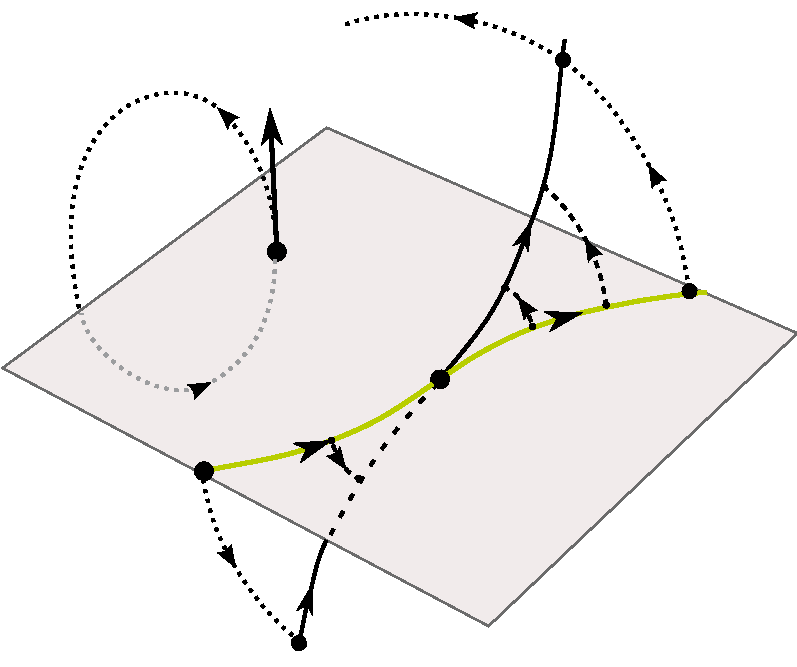
\includegraphics[width=\unitlength]{ReducTraj5.pdf}}%
   \put(0.06854399,0.36282057){\color[rgb]{0,0,0}\rotatebox{-30.34758661}{\makebox(0,0)[lb]{\smash{$\pSRed$}}}}%
   \put(0.57768586,0.29773425){\color[rgb]{0,0,0}\rotatebox{0.0313674}{\makebox(0,0)[lb]{\smash{$\sspRed(0)$}}}}%
   \put(0.59310014,0.69932675){\color[rgb]{0,0,0}\rotatebox{0.03136739}{\makebox(0,0)[lb]{\smash{$\ssp(\zeit)$}}}}%
   \put(0.8268425,0.39772328){\color[rgb]{0,0,0}\rotatebox{0.03136739}{\makebox(0,0)[lb]{\smash{$\sspRed(\zeit)$}}}}%
   \put(0.81220962,0.66529577){\color[rgb]{0,0,0}\rotatebox{0.03136739}{\makebox(0,0)[lb]{\smash{$\LieEl(\theta(\zeit))\ssp(\zeit)$}}}}%
   \put(0.21150193,0.63610779){\color[rgb]{0,0,0}\rotatebox{0.0313674}{\makebox(0,0)[lb]{\smash{$\LieEl\,\slicep$}}}}%
   \put(0.37740434,0.49597258){\color[rgb]{0,0,0}\rotatebox{0.0313674}{\makebox(0,0)[lb]{\smash{$\slicep$}}}}%
   \put(0.3627714,0.69665188){\color[rgb]{0,0,0}\rotatebox{0.0313674}{\makebox(0,0)[lb]{\smash{$\sliceTan{}$}}}}%
 \end{picture}%
\end{center}
\caption{\label{f-ReducTraj1}The \slicePlane\ \pSRed\ is a hyperplane % \refeq{PCsect0}
passing through the {\template} point $\slicep$
and normal to its group tangent $\sliceTan{}$.
It intersects all group orbits (dotted lines) in an open
neighborhood of $\slicep$.  The full \statesp\ trajectory $\ssp(\tau)$ (solid black line) and the \reducedsp\
trajectory $\sspRed(\zeit)$ (solid green line) belong to the same group orbit
$\pS_{\ssp(\zeit)}$ and are equivalent up to a group rotation
$\LieEl\left(\theta(\zeit)\right)$ (from \wwwcb{}).
}%
\end{figure}

Reduced trajectories $\sspRed (t)$ can be obtained in two ways: by post-processing data
or by reformulating the dynamics and integrating directly on the \slice. In the post-processing method, which can be applied to both numerical and experimental data,
one takes the data in the full \statesp\ and looks for the time dependent group parameter
that brings the trajectory $\ssp(\zeit)$ onto the \slice. That is, one finds $\theta (\zeit)$ such that $\sspRed(\zeit) = \LieEl(- \theta (\zeit)) \ssp (\zeit)$
satisfies the \slice\ condition:
\beq
\braket{\sspRed(\zeit) - \slicep}{\sliceTan{}} = 0
\,.
\ee{SliceCond}

In the second method, one reformulates the dynamics (for Abelian groups) as
\begin{subequations}\label{eq:so2reduced}
  \beq\label{eq:intSlice}
	\velRed(\sspRed) = \vel(\sspRed)
	-\dot{\theta}(\sspRed) \, \groupTan(\sspRed)
  \eeq
  \beq\label{eq:reconstruction}
	\dot{\theta}(\sspRed) = {\braket{\vel(\sspRed)}{\sliceTan{}}}/
				{\braket{\groupTan(\sspRed)}{\sliceTan{}}}
  \, ,
  \eeq
\end{subequations}
and computes $\sspRed (\zeit)$ and $\theta (\zeit)$ directly. In \refeq{eq:so2reduced}, $\velRed$ is the projection
of the full \statesp\ velocity \vel(\ssp) onto the \slicePlane. For a detailed derivation
of \refeq{eq:so2reduced}, see \refref{DasBuch}. Note that the time derivative
of the group parameter, which also appears in $\velRed$,
becomes singular if the dot product $\braket{\groupTan(\sspRed)}{\sliceTan{}}$
vanishes. We will refer the set of points on the \slicePlane\ which satisfy
\beq
\braket{\groupTan(\sspRed^*)}{\sliceTan{}} = 0
\,
\ee{ChartBordCond}
as the \emph{\sliceBord}.

%In general, \chartBord\ can be avoided by use of
%multiple \template s and arranging them in a way that the trajectories do not
%intersect the \chartBord , as done in \refref{atlas12}. In the particular
%case of the \twoMode\ system that we study in this paper, we can describe
%the reduced dynamics using a single \slice\ by picking a \template\ for which
%the \chartBord\ is a flow invariant subspace, hence never visited.

%If a $d$\dmn\ dynamical flow is $\Group$-equivariant under actions of
%an $N$ continuous parameters symmetry group $\Group$, its $d$\dmn\ \statesp\ is foliated
%by $N$\dmn\ group orbits, and the symmetry-\reducedsp\
%$\pS/\Group$ is $(d\!-\!N)$\dmn.
%The simplest continuous symmetry groups are the 1-parameter compact rotation
%group $\SOn{2}$ and the 1-parameter noncompact translation group
%$T(1)$; here we shall focus on the $\SOn{2}$ case.

So far, we have not put any constraints on the symmetry group that we are quotienting,
beyond the requirement that it be Abelian\ES{2015-05-20}{Maybe you should discuss why
you imposed the restriction on Abelian groups.}.
From here on, we restrict our discussion to 1-parameter compact $\SOn{2}$
rotations that arise in spatially extended systems. \DBedit{In order to construct
a representation for $\SOn{2}$}
\DB{2014-05-15}{What are we trying to say exactly here? Also does it make
sense to make the function z and its coefficient $z_k$ so that the
notation is consistent with the discussion about slice fixing in
\refsect{s-slice2modes}}
let us take a Fourier series expansion of a real valued smooth periodic
function:
\beq
	z(x,\zeit) = \sum\limits_{k=- \infty}^\infty z_k\left(\zeit\right) e^{i k x}, \,\,\,z_k = x_k + i y_k.
\ee{FourierSeries}
Truncating the expansion to $m$ modes, we
write the real and imaginary parts of the Fourier coefficients with
$k \geq 1$ as the state vector $\ssp = (x_1, y_1, x_2, y_2,..., x_m, y_m)$. The action of the $\SOn{2}$ group on this vector
can then be expressed as a block diagonal matrix:
%More explicit form, does not fit in a column:
%\beq
	 %\LieEl (\theta)= \\
					  %\begin{pmatrix}
					  %\cos \theta & \sin \theta & 0               & 0              & \cdots & 0              & 0               \\
					 %-\sin \theta & \cos \theta & 0               & 0              & \cdots & 0              & 0               \\
					  %0             & 0 		   & \cos 2 \theta & \sin 2 \theta & \cdots & 0              & 0               \\
					  %0             & 0            &-\sin 2 \theta & \cos 2 \theta & \cdots & 0              & 0               \\
					  %\vdots       & \vdots      & \vdots         & \vdots        & \ddots & \vdots         & \vdots         \\
					  %0             & 0 		   & 0               & 0              & \cdots & \cos m \theta & \sin m \theta  \\
					  %0             & 0            & 0	             & 0              & \cdots &-\sin m \theta & \cos m \theta
					  %\end{pmatrix}
%\eeq
\beq
	\LieEl(\theta) = \begin{pmatrix}
						R(\theta) & 0 			  & \cdots & 0 \\
						0		   & R(2 \theta) & \cdots & 0 \\
						\vdots	   & \vdots 	  & \ddots & \vdots \\
						0		   & 0	          & \cdots & R (m \theta)
					   \end{pmatrix} ,
\ee{mmodeLieEl}
where
\beq
	R(n \theta) =	\begin{pmatrix}
					\cos n \theta & - \sin n \theta \\
					\sin n \theta & \cos n \theta
					\end{pmatrix}
\ee{rotationmatrix}
is the rotation matrix for $n$th Fourier mode.
The Lie algebra generator for $\LieEl(\theta)$ is given by
\beq
	 \Lg =  \begin{pmatrix}
			 0 & -1 & 0 & 0 & \cdots & 0 & 0 \\
			 1 & 0 & 0 & 0 & \cdots & 0 & 0 \\
			 0 & 0 & 0 & -2 & \cdots & 0 & 0 \\
			 0 & 0 & 2 & 0 & \cdots & 0 & 0 \\
			 \vdots & \vdots & \vdots & \vdots & \ddots & \vdots & \vdots \\
			 0 & 0 & 0 & 0 & \cdots & 0 & -m \\
			 0 & 0 & 0 & 0 & \cdots & m & 0
			 \end{pmatrix} .
\ee{mmodeLg}

In order to construct a \slicePlane\ for such a system, let us choose the following \slice\ \template:
\beq
	\slicep = (1, 0, ..., 0) .
\ee{firstmodetemp}
The \slice\ condition \refeq{SliceCond} then constraints points on the reduced trajectory to the hyperplane given by
\beq
	\sspRed = (\hat{x}_1, 0, \hat{x}_2, \hat{y}_2, ..., \hat{x}_m, \hat{y}_m) .
\ee{slicetemp}
In order to satisfy the requirement that group orbits cross the \slice\ once and only once, we also restrict the \slicePlane\ to the half-space where $\hat{x}_1 > 0$.
Without this requirement group orbits would pierce the \slicePlane\ twice.
In general, a \slicePlane\ can be constructed by following a similar procedure for any choice of \template, allowing the symmetry
reduction of the dynamics in a neighborhood of the \template\ bounded by the \sliceBord\ \refeq{ChartBordCond}.
However, the power of choosing template \refeq{firstmodetemp} becomes apparent by analyzing the border of its \slicePlane.
The points on \refeq{slicetemp} only lie on the \sliceBord\ if $\hat{x}_1 = 0$.
This means that as long the dynamics are such that the magnitude of the first mode never vanishes,
\emph{every} group orbit is guaranteed to have a unique representative point on the \slicePlane.

\footnote{Note that, in general, any template of the form $\slicep = (\hat{x}'_1, \hat{y}'_1, 0,...,0)$ would work just as well since the first mode has the symmetry of a circle. We picked the \slice\ \template\
\refeq{firstmodetemp} for computational convenience.}
%

The \template\ \refeq{firstmodetemp} for $\SOn{2}$ was introduced by
Budanur~\etal\rf{BudCvi14},
and is different from those used in the previous implementations
of the \mslices,\rf{rowley_reconstruction_2000,BeTh04,SiCvi10,FrCv11,atlas12,ACHKW11} in the sense that it is solely geometrical and it does
not necessarily carry any information about the dynamics
\ES{2014-05-20}{It's always a good idea to read the papers that we cite,
even though nowadays it's not mandatory (it seems).
The \template\ \refeq{firstmodetemp} is used in Sect. 6.2 of SiCvi10,
where it is called ``irreducible subspace slice.'' Moreover, you should
have a look at Olver\rf{OlverInv} (and cite\rf{FelsOlver98,OlverInv}
for the postprocessing approach). Their typical choice of a slice is equivalent
to using \template\ \refeq{firstmodetemp}. }.
More insight can be
gained by writing the symmetry-reduced evolution equations \refeq{eq:so2reduced}
explicitly for the template \refeq{firstmodetemp}:
\begin{subequations}
\beq
\velRed ( \sspRed )  = \vel(\sspRed)
   - \frac{\dot{y}_1\left(\sspRed\right)}{\hat{x}_1} \, \groupTan(\sspRed)
\label{e-so2red1stmode}
\,.
\eeq
\ESedit{
  \beq\label{eq:reconstruction1stmode}
	\dot{\theta}(\sspRed) = \frac{\dot{y}_1(\sspRed)}{\hat{x}_1}
  \, ,
  \eeq
}
\end{subequations}
\ESedit{
Noting that the angle of a point $(x_1,y_1)$ in the first Fourier mode plane is $\phi_1=\tan^{-1}\frac{y_1}{x_1}$,
we find
\beq
  \dot{\phi}_1 = \frac{x_1}{r_1^2}\dot{y}_1-\frac{y_1}{r_1^2}\,\dot{x}_1\,,
\eeq
where $r_1^2=x_1^2+y_1^2$. Noting that on the slice, $\hat{y}_1=0$, we arrive at
\beq\label{eq:phi1}
  \dot{\theta}(\sspRed) = \dot{\phi}_1(\sspRed)\,.
\eeq
That is, for our choice of \template\ \refeq{firstmodetemp}, the reconstruction phase coincides with
the first Fourier mode phase.
}
\ES{2014-05-20}{What would you think about introducing a functional
notation for $y_1$ as in \refeq{eq:reconstruction1stmode}?}
\PC{2014-05-25}{We should copy and paste from \refref{BudCvi14} all stuff
about the in-slice time here? }


In general, one must be careful when the dynamics approach the \slice\ border $\hat{x}_1 = 0$. When this happens
the near-divergence of $\velRed$ can be regularized by introducing a rescaled time coordinate such that
$d\hat{\zeit} = d\zeit / \hat{x}_1$\rf{BudCvi14}. However, in our study of the \twoMode\ system, we omit this
step since points with a vanishing first mode correspond to an invariant subspace of the flow and hence are never visited by the dynamics.

\subsection{Postproccessing approach}
\label{s-slice2modes}

\ES{2014-05-15}{This section refers to the ``method of moving frames'' (postprocessing approach)
and as such belongs here. It has to be generalized a bit (I will do it if you agree with the change).
Second mode \slice\ can be used also for integration on the \slice\ and can be introduced earlier.
}

\begin{figure}%[H]
\centering
 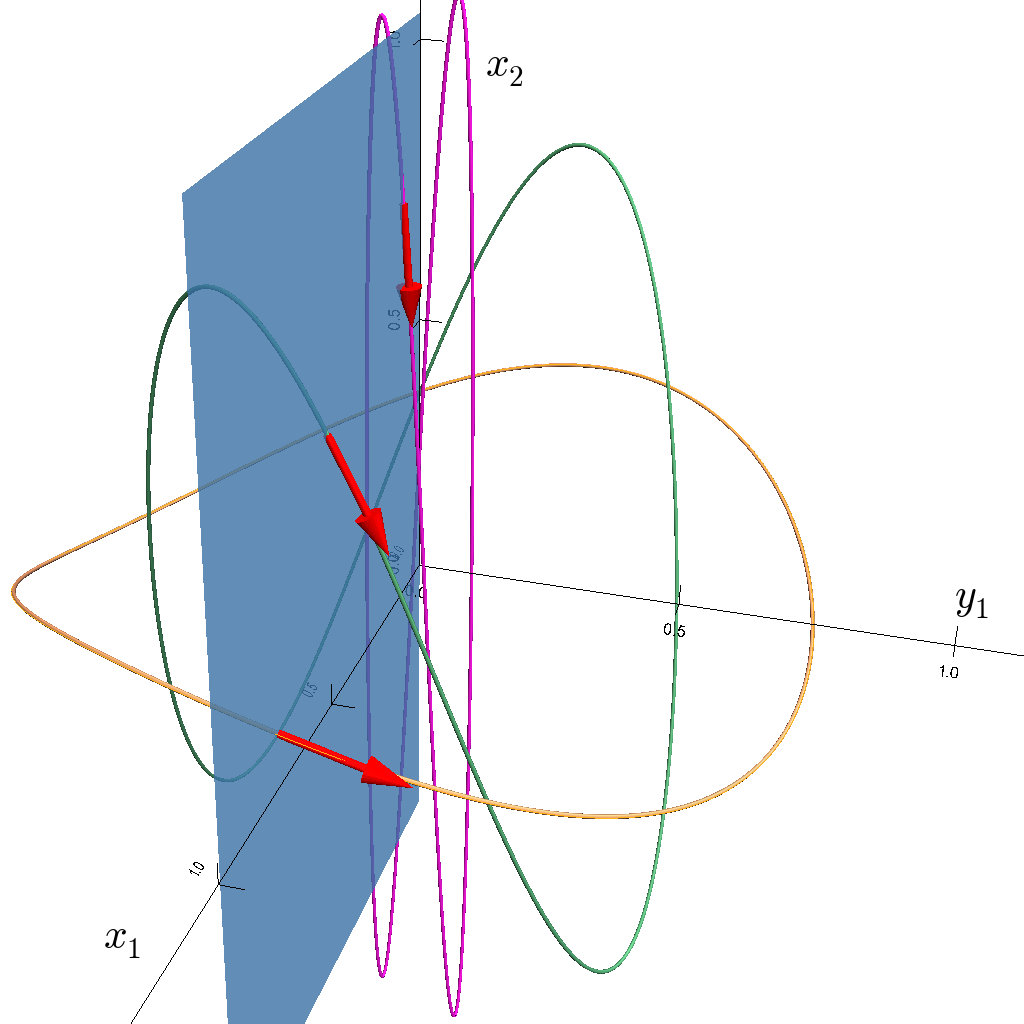
\includegraphics[width=0.45\textwidth]{BBgorbitsandslice}
\caption{$\SOn{2}$ Group orbits of \statesp\ points $(0.75, 0, 0.1, 0.1)$ (orange), $(0.5, 0, 0.5, 0.5)$ (green)
$(0.1, 0, 0.75, 0.75)$ (pink) and the first mode \slicePlane\
\refeq{slicetemp} (blue). The group tangents at the intersections with the \slicePlane\ are shown as red arrows.
As the magnitude of the first Fourier mode becomes small relative to the magnitude of the second one, the group tangent becomes more parallel to the \slicePlane.}
\label{fig:BBgorbitsandslice}
\end{figure}

In \refsect{s-slice}, we explained the general procedure for reducing
the \SOn{2} symmetry by \mslices. Here, we focus on its
geometrical interpretation using the \twoMode\
system as an example. The \slice\ defined by \refeq{firstmodetemp} and the directional
constraint $\hat{x}_1 > 0$
%
\DB{2014-05-15}{Think this should be $\hat{x}_1$. Revert to $x_1$ if I'm wrong.}
%
fix the phase of the first complex Fourier mode to $0$. \Statesp\ points are related to their representative points on the \slicePlane\ by the following $\Un{1}$ action:
\beq
	\sspRedC_n = e^{-\ii n \phi_1} \sspC_n \, .
\ee{e-1stmodeTransform}
\DBedit{We immediately see that the reconstruction phase in \refeq{eq:so2reduced}
is, for this particular \slice, the phase of the first mode without the
symmetry reduction.}
%
\DB{2014-05-15}{I don't immediately see what we are saying here. How does
this relate to \refeq{eq:so2reduced}? I think this needs better
explanation.}
\ES{2014-05-15}{It's not straightforward to see this, also for me, unless
I think of the postprocessing approach. So I have added \refeq{eq:phi1}
above. Please check and discuss in the blog if needed.}
%
The relation \refeq{e-1stmodeTransform} provides us
another interpretation for the \sliceBord :  For the template \refeq{firstmodetemp},
the \sliceBord\ condition \refeq{ChartBordCond} yields,
$|\sspRedC_1| = |\sspC_1| = 0$, which means that the phase of the first Fourier
mode \BBedit{and hence \DBedit{the transformation \refeq{e-1stmodeTransform}
is not defined.}}
%
\DB{2014-05-15}{This phrase has no meaning.}
\BB{2014-05-15}{Is it better know?}
%
This is illustrated in \reffig{fig:BBgorbitsandslice}, which shows $3D$ projections of the
group orbits and group tangents of three reduced \statesp\ points. As the magnitude of the
first mode, $\sqrt{\hat{x}_1^2 + \hat{y}_1^2}$, relative to that of the second mode becomes smaller,
its group tangent has a larger component parallel to the \slicePlane. The \sliceBord\ condition
\refeq{ChartBordCond} is satisfied when the group tangent becomes parallel to the \slicePlane.
%
\DB{2014-05-15}{Don't love my wording of ``parallel to the \slicePlane'' since some people might interpret the
\slicePlane\ as being defined by a vector normal to its surface and hence a perpendicular to the
group tangent at the \sliceBord. However, I think that ``component that lies within the slice'' is
sort of vague and not well defined mathematically. What do you guys think?}


An immediate generalization of the transformation \refeq{e-1stmodeTransform},
is to fix the phase of a higher Fourier mode rather than that of the first one; this, however, requires
some extra care as we shall explain for the second Fourier mode.
Consider the phase-fixing transformation,
\beq
	\sspRedC_n = e^{-\ii n \frac{\phi_2}{2}} \sspC_n \, ,
	\label{e-2ndmodeTransform}
\eeq
which fixes the phase of the second mode to $0$. Note, however, that since
$\phi_2 \in (0, 2 \pi]$ it can have discontinuities of $2 \pi$. This means
that when the first Fourier mode is transformed, it will have a phase discontinuity
of $\pi$. This discontinuity can be fixed by another
transformation:
\bea
	\tilde{\sspC}_1 &=& e^{-\ii 2 \hat{\phi}_1} |\sspRedC_1 | \, , \continue
	\tilde{\sspC}_{n \neq 1} &=& \sspRedC_n \, ,
	\label{e-PhaseDoubling}
\eea
where we simply doubled the phase $\hat{\phi}_1$ of the symmetry-reduced
first mode $\sspRedC_1$, obtained by \refeq{e-2ndmodeTransform} and left
the rest of the modes unchanged. Combination of \refeq{e-2ndmodeTransform}
and \refeq{e-PhaseDoubling} is a valid symmetry reduction scheme since every
group orbit is represented by a single point, furthermore, it is also continuous
and revertible hence one can make further computations, such as constructing
Poincar\'{e} sections, using this form. For the 2-mode case at hand, representation
\refeq{e-PhaseDoubling} does not have any particular advantage against
\refeq{e-1stmodeTransform}, however, for higher dimensional flows, second
(or higher) Fourier mode subspaces can have dynamical importance as shown in
\refref{SCD07}. In order to capture those regions of the \statesp\ this
representation would be a useful alternative.

\subsection{Polar coordinates}
\label{s-polar}

In \refref{PoKno05}, a polar coordinate representation of \refeq{eq:DangSO2}
is obtained by defining the $\LieEl$-invariant phase: $\Phi = \phi_2 - 2 \phi_1$
and three symmetry invariant coordinates $(r_1, r_2 \cos \Phi, r_2 \sin \Phi)$.
One can see by direct comparison with \refeq{e-1stmodeTransform}, which
yields $\sspRedC_1 = r_1$ and $\sspRedC_2 = r_2 e^{\ii \Phi}$, that this
representation is a special case $(m=2)$, of the \slice\ defined by
\refeq{firstmodetemp}. Corresponding ODEs for the polar representation
were obtained in \refref{PoKno05} by  chain rule and substitution. Note
that \mslices\ provides a general form \refeq{e-so2red1stmode} for symmetry
reduced time evolution.

%           %experimenting with svn-multi

\svnkwsave{$RepoFile: siminos/froehlich/flow.tex $}
\svnidlong {$HeadURL$}
{$LastChangedDate$}
{$LastChangedRevision$} {$LastChangedBy$}
\svnid{$Id$}


\chapter{\CLf}
\label{chap:blog}

     \Private{
\noindent{\bf Rebecca -
Jun 16 - Aug 21 2009}:\\
     }
This project first reproduces results reported by
Siminos\rf{SiminosThesis}, and then investigates various ways
of `quotienting' the \SOn{2} symmetry of \cLe, and reducing
the dynamics to symmetry 4-dimensional \reducedsp.
     \PC{
   When you write
   a project report or a research article, you always write abstract, introduction
   and conclusions first, and then keep rewriting them often.
   They are the most important parts of the text, as that is
   for most people only parts they will look at.
   }


The project consists of my notes and exercises. The flow of
the argument is in the classical
\HREF{http://en.wikipedia.org/wiki/Socratic_method}{Socratic dialogue}
mode; question, answer, question, $\cdots$.
    %
    \Private{ % subversion label pages
$\footnotemark\footnotetext{{\tt \svnkw{RepoFile}}, rev. \svnfilerev:
 last edit by \svnFullAuthor{\svnfileauthor},
 \svnfilemonth/\svnfileday/\svnfileyear}$
    } % end \Private{

The \cLe\ were introduced by Gibbon and McGuinness\rf{GibMcCLE82}
as a low-dimensional model of baroclinic instability in the
atmosphere. In the complex form, they are given by
\beq
\begin{split}
 \dot{x} &=-\sigma x+ \sigma y \\
 \dot{y} &=(r-z)x-a y \\
 \dot{z} &= \frac{1}{2}\left(x y^*+x^*y\right)-b z\,
 \label{eq:CLe}
\end{split}
\eeq
where $x,y$, $r=r_1+ i\,r_2$, $a=1+i\,e$ are complex and $z$,
$b$, $\sigma$ are real. Rewritten in terms of real variables
$x=x_1+ i\, x_2\,,\ y=y_1+i\, y_2$, \cLe\ are a 5-dimensional
first order ODE system\rf{SiminosThesis}
\beq
\begin{split}
	\dot{x}_1 &= -\sigma x_1 + \sigma y_1\\
	\dot{x}_2 &= -\sigma x_2 + \sigma y_2\\
	\dot{y}_1 &= (r_1-z) x_1 - r_2 x_2 -y_1-e y_2 \\
	\dot{y}_2 &= r_2 x_1 + (r_1-z) x_2 + e y_1- y_2\\
	\dot{z} &= -b z + x_1 y_1 + x_2 y_2\,.
	\label{eq:CLeR}
\end{split}
\eeq
In all numerical calculations that follow we shall set the
parameters to the Siminos values\rf{SiminosThesis},
\beq
r_1=28,\; b=\frac{8}{3},\;
\sigma=10,\; e=\frac{1}{10},\quad \mbox{and} \quad r_2=0
\,.
\ee{SiminosPrmts}

Here we are not interested in the physical applications of
these equations; rather, we study them as a simple example of
a dynamical system with continuous (but no discrete)
symmetries. Our goal is to find computationally
straightforward method of reducing the dynamics to a
lower-dimensional \statesp, where each group orbit of the
full system (\ie, set of translationally equivalent states)
is represented by a single point. If successful, the methods
that we develop might be applicable to very high-dimensional
flows, such as translationally equivariant fluid flows
bounded by pipes or planes\rf{GHCW07,GibsonMovies}.

\noindent {\bf Acknowledgments.}
S.F. work was supported by the National Science Foundation
grant DMR~0820054.
P.C. thanks Glen Robinson Jr. for support.

\subsection{Visualizing \cLf}

In \refexer{exer:PlotCLf} we simulate \cLf\ in order to
visualize its long-time dynamics, as in
\reffig{fig:CLEx1x2z}. The dynamics is a big mess - the
trajectory seems to oscillate while drifting around $z$-axis.
Of most importance in \reffig{fig:CLEx1x2z}, is to notice
that the flow has a rotational symmetry about the $z$-axis.
Throughout the rest of the project we will try to find more
illuminating ways of understanding the dynamics of this flow
as well as ways of "cleaning it up"--that is, removing this
symmetry and reducing the ODE system from five dimensions to
four.
%    \PC{label axes, use legible fonts in all figures.}
%    \PC{put all single figures into SFIG format, as
%        \reffig{fig:CLEx1x2z}.}
                                                    \exerbox{exer:PlotCLf}

%%%%%%%%%%%%%%%%%%%%%%%%%%%%%%%%%%%%%%%%%%%%%%%%%%
% computed by graphs.nb
\SFIG{CLEx1x2z}
{}{
A typical $\{x_1,x_2,z\}$ plot of the \cLf\ strange attractor,
with initial point
$(x_1, x_2, y_1, y_2, z) = (1, 0, 0, 1, 1)$.
    }{fig:CLEx1x2z}
%%%%%%%%%%%%%%%%%%%%%%%%%%%%%%%%%%%%%%%%%%%%%%%%%%


\section{Linear stability}
\label{sect:stability}
%\PC{Write up here the general text on stability, following \refref{DasBuch},
%\\
%\wwwcb{/chapters/stability.pdf}
%    }
In our first attempt to understand the dynamics of the flow, we examine its stability by finding the stability matrix $\Mvar$. This is the matrix of partial derivatives of $v(x)$,
\beq
\Mvar = \frac{\pde v}{\pde x}=
\left(\barr{ccccc}\medskip
\frac{\pde\dot{x}_1}{\pde x_1} & \frac{\pde\dot{x}_1}{\pde x_2} &\frac{\pde\dot{x}_1}{\pde y_1} & \frac{\pde\dot{x}_1}{\pde y_2} & \frac{\pde\dot{x}_1}{\pde z}\\\medskip
\frac{\pde\dot{x}_2}{\pde x_1} & \frac{\pde\dot{x}_2}{\pde x_2} &\frac{\pde\dot{x}_2}{\pde y_1} & \frac{\pde\dot{x}_2}{\pde y_2} & \frac{\pde\dot{x}_2}{\pde z}\\\medskip
\frac{\pde\dot{y}_1}{\pde x_1} & \frac{\pde\dot{y}_1}{\pde x_2} &\frac{\pde\dot{y}_1}{\pde y_1} & \frac{\pde\dot{y}_1}{\pde y_2} & \frac{\pde\dot{y}_1}{\pde z}\\\medskip
\frac{\pde\dot{y}_2}{\pde x_1} & \frac{\pde\dot{y}_2}{\pde x_2} &\frac{\pde\dot{y}_2}{\pde y_1} & \frac{\pde\dot{y}_2}{\pde y_2} & \frac{\pde\dot{y}_2}{\pde z}\\
\frac{\pde\dot{z}}{\pde x_1} & \frac{\pde\dot{z}}{\pde x_2} &\frac{\pde\dot{z}}{\pde y_1} & \frac{\pde\dot{z}}{\pde y_2} & \frac{\pde\dot{z}}{\pde z}\\
\earr\right)
\label{5x5stabMat}
\eeq
For the \cLe\ it is the $[5\!\times\!5]$ matrix,
                                                    \exerbox{exer:StabmatCLf}
\beq
  \Mvar =\left(\barr{ccccc}
    -\sigma    	& 0 		& \sigma & 0    &  0 \\
	0 	& -\sigma       & 0      & \sigma   &  0 \\
	r_1-z  &     -r_2      & -1     & -e & -x_1 \\
	r_2     & r_1-z       	& e  	& -1       & -x_2 \\
	y_1     & y_2           & x_1    & x_2      & -b
    \earr\right)
\eeq
As explained in ChaosBook.org\rf{DasBuch}, a stability matrix
describes the instantaneous rate of shearing of the
infinitesimal neighborhood of $x(t)$ by the flow. That is, it
describes how quickly points initially very near to $x(t)$ will
diverge away from it in time. It is the matrix of
velocity gradients. This matrix $\Mvar$ is also an important
tool which we will use later on.


\section{\Eqva}

An \eqv\ $\EQV{}$ is a point $\ssp_{\EQV{}}$ for which the
velocity field of an ordinary differential equation
$\dot{\ssp} = v(\ssp)$ is zero, $v(\ssp_{\EQV{}})=0$. These
are points where the flow does not move, and if it reaches an
equilibrium, the flow remains there. For the \cLe\, the only
equilibrium we found was at the origin $\EQV{0}=(0, 0, 0, 0,
0)$. If we could set this {\em infinitely precisely} as the
initial point of the flow, instead of seeing the messiness of
\reffig{fig:CLEx1x2z}, we would stay at this single point for
all times. In any simulation, the (finite precision)
trajectory eventually leaves this point.
                                                    \exerbox{exer:EquiCLe}

\subsection{Stability of \eqva}
At an equilibrium, the flow manages to stay at a single
point, but what if we start at points near the equilibrium? Will
they collapse into the equilibrium, or will they diverge away
from it? In order to answer this, we find and examine the
eigenvalues and eigenvectors of \Mvar\ evaluated at the
equilibrium $\EQV{0}$.
                                                    \exerbox{exer:EigenE0}
For the \cLe\, we find that the eigenvalues are
        \PC{ChaosBook convention is to order eigenvalues
        from most positive (unstable) to the most negative,
        that is why I renumbered them. Try to follow that
        everywhere. Replace complex eigenvectors by the real,
        imaginary parts, as that is what you actually use - I
        did this in \refeq{eigVecQ1}. I might have introduced
        errors in renumbering them, so trust your own
        computations, especially regarding the
        \reffig{fig:CLEE0} comments.
        }
\beq
\begin{split}
\lambda_{1,2} &=11.8277 \pm 0.062985 i\\
\lambda_{3,4} &=-22.8277 \pm 0.037015 i\\
\lambda_5 &=-2.66667\\
\end{split}
\eeq
with the associated eigenvectors
    \PC{\label{suspectEigVecs}is suspect:
    real, im parts seem interchanged in $e_1$?}
\bea
e_{1} &=& e_2^* =(0.001321+0.4581 i, 0.4581-0.001321 i, i, 1, 0)
\label{suspectEigVecs}\\
e_3 &=& e_4^* = (0.002249-0.7795 i, -0.7795-0.002249 i, 2.8421+i, 1, 0)
\continue
e_5 &=& (0, 0, 0, 0, 1)
\,.
\nnu
\eea
By examining the eigensystem, we can get a sense of what
happens to points near the equilibrium $\EQV{0}$. The
numerical values of the real parts of the eigenvalues
determine how quickly the flow will converge onto or diverge
away from the equilibrium. For a positive real part the flow
will diverge, and for a negative real part it will converge.
Complex eigenvalues also indicate that the motion will be
spiraling.

For the \cLe\ equilibrium $\EQV{0}$, the values of the
imaginary parts are orders of magnitude smaller than the real
parts, so that there will be very little spiraling. The large
values of the real parts tell us that the flow will
diverge/converge from the equilibrium very quickly.
                                                    \exerbox{exer:PlotEigenE0}

To illustrate this, we plot the eigenvectors (as real and
imaginary parts) and the flow at initial points very close to
$\EQV{0}$. The two real vectors (corresponding to a single
complex eigenvector) define the plane in which the flow will
spiral. We initiate the flow very close to $\EQV{0}$ at a
point along one of these vectors. In \reffig{fig:CLEE0},
    \RW{
    I'm still having trouble with this figure and
    matching up it's eigenvalues. In the Mathematica notebook
    where it was computed (eigensystem.nb), the "yellow"
    eigenvectors that are plotted are labeled $e3$, which
    numerically matches the second vector in the list of computed
    eigenvectors (at the time, we called the all-real vector
    $e1$). The second eigenVALUE which would correspond to this
    yellow-$e3$ vector is -22... Predrag says it should be the
    +11...eigenvalue, but I can't find how they match up
    correctly. I have double and triple-checked all of the
    subscripts and as far as I can tell, the vectors in the plot
    are $e_4$, as listed here in this paper (not the $e4$ in
    Mathematica) and have eigenvalue -22. Will continue on
    ignoring this problem, I'm hoping I just missed something.
    }
we can see that for the vectors with a very small imaginary
part and a positive real part, the flow does not spiral
noticeably and that it diverges away from the equilibrium very
quickly.
%%%%%%%%%%%%%%%%%%%%%%%%%%%%%%%%%%%%%%%%%%%%%
% computed by eigensystem.nb
\SFIG{ProblemsPill} %CLEE0}
{}{
$\{x_1, x_2, z\}$ plot of the expanding eigenvector $e_1$
(red) and the contracting eigenvector $e_4$ (yellow) of the
\eqv\ $E_0$ \stabmat\ of \cLf, with initial point at $\frac{1}{100}
e_4$.
}
{fig:CLEE0}
%%%%%%%%%%%%%%%%%%%%%%%%%%%%%%%%%%%%%%%%%%%%%


\section{Symmetries of dynamics}
\label{sect:SymmDyn}

         \Private{
\noindent{\bf Rebecca -
Jun 18 2009}:\\
\medskip\noindent
         }
In order to eventually remove the rotational symmetry in the
\cLf\, we need to show that the flow is rotationally
equivariant. By showing this, we will then be able to apply
algorithms to remove the symmetry. Rotational equivariance in
this situation will let us commute a rotation operator with
taking time derivatives.\RW{I plan on writing more here, just
haven't thought of what else I want to say yet.}

We begin by defining `equivariance.'
A flow $\dot{x}= v(x)$ is equivariant under an operation $\mathbb{G}$ when
\beq
\mathbb{G} \cdot v(x)=v(\mathbb{G} \cdot x)
\,.
\ee{eq:FiniteRot}
A Lie group element relating different \statesp\ points by a
linear continuous symmetry operation can be written as
\beq
\mathbb{G}(\theta)=e^{{\theta} \Lg }
\,.
\ee{FiniteRot}
                                                    \exerbox{exer:FinRot2d}
For an infinitesimal rotation, $\theta \ll 1$,
\[
\mathbb{G}(\theta)=1+\theta  \Lg  + \cdots
\,,
\]
the statement of equivariance
$
\dot{x}=\mathbb{G}^{(-1)} \cdot v(\mathbb{G} \cdot x)
$
becomes
\[
\dot{x}=(1-\theta \Lg ) \cdot v(x+\theta  \Lg \cdot x) + \cdots
       =v(x)-\theta \left(
            \Lg \cdot v(x) - \frac{dv}{dx} \cdot \Lg \cdot x
                     \right)  + \cdots
\,.
\]
The $\dot{x}$ and $v(x)$ cancel, and the $\theta$ can be
divided out. We are left with the {\em infinitesimal
rotations} version of the equivariance condition
\refeq{eq:FiniteRot}:
\beq
0=- \Lg \cdot v(x)+\Mvar \cdot \Lg \cdot x
\,,
\label{eq:InfnmslRot}
\eeq
where $\Mvar = \frac{\pde v}{\pde x}$ is the \stabmat\ \refeq{5x5stabMat}.

We have used both this infinitesimal rotation condition and
the finite angle rotation condition \refeq{eq:FiniteRot}, to
verify that the \cLe\ are rotationally equivariant.
                                                    \exerbox{exer:InfinRotInvari}
                                                    \exerbox{exer:FinRotInvarCmplx}
                                                    \exerbox{exer:FinRotInvari}


\section{\Reqva}

To further visualize the drifting of the flow around the
$z$-axis, we next find and plot the relative equilibria of
the \cLe. A relative equilibrium is a solution of the flow
which appears stationary in a frame rotating at the
appropriately chosen constant angular velocity. We find these
points in a manner similar to finding the equilibria, with
one difference. As the flow drifts (rotates), a relative
equilibrium will drift as well, so that instead of setting
all of the $v(x)=0$, we allow the component of $v(x)$ tangent
to direction of group rotation to be non-zero. This tangent is not
necessarily easily defined in the
Cartesian coordinates which we have so far been using. The
relative equilibrium is more conveniently determined  in
polar coordinates.

\subsection{Equations in the polar form}
\label{sect:coordChange}
\PC{Gilmore and Letellier\rf{GL-Gil07b} is a good reference
        for a discussion of such coordinate changes}
We can rewrite the \cLe\ to polar coordinates using the definition
\beq
(x_1,x_2,y_1,y_2,z) =
    (\rho_1 \cos\theta_1,\rho_1\sin\theta_1,
     \rho_2\cos\theta_2,\rho_2\sin\theta_2,z)
\,,
\label{eq:CartToPol}
\eeq
and come up with the new equations
\[ %\beq
\left(
\begin{array}{c}
\dot{\rho}_1\\
\dot{\theta}_1\\
\dot{\rho}_2\\
\dot{\theta}_2\\
\dot{z}
\end{array}
\right)
=
\left(
\begin{array}{c}
 -\sigma\left(\rho_1 - \rho_2\cos\theta\right) \\
 -\sigma\frac{\rho_2}{\rho_1}\sin \theta  \\
 -\rho_2 + \rho_1\left((r_1-z)\cos \theta - r_2 \sin\theta\right)\\
  e  + \frac{\rho_1}{\rho_2}\left((r_1-z)\sin\theta +r_2 \cos\theta\right)\\
 -b z + \rho_1\rho_2\cos\theta
\end{array}
\right)
,
\] %\ee{eq:PolarCLe}
                                                    \exerbox{exer:HarmOscPolar}
                                                    \exerbox{exer:polarCLe}
We know from classical mechanics that for translationally or
rotationally invariant flows the relative distance is
invariant (that is why one speaks of `relative' equilibria),
hence we introduce a variable $\theta = \theta_1-\theta_2$.
This is the variable which allows us to
ultimately find the relative equilibria. As the flow is
rotating, $\theta_1$ and $\theta_2$ are changing, but, at the
relative equilibria, the difference between them is constant.
This new variable also allows us to rewrite the \cLe\ yet
again, this time in only four dimensions.
\beq
\left(
\begin{array}{c}
\dot{\rho}_1\\
\dot{\rho}_2\\
\dot{\theta}\\
\dot{z}
\end{array}
\right)
=
\left(
\begin{array}{c}
 -\sigma\left(\rho_1 - \rho_2\cos\theta\right) \\
 -\rho_2 + (r_1-z)\rho_1\cos \theta\\
  -e -\left(\sigma\frac{\rho_2}{\rho_1}
 +(r_1-z)\frac{\rho_1}{\rho_2}\right)\sin\theta\\
 -b z + \rho_1\rho_2\cos\theta
\end{array}
\right)
\label{eq:PolarCLeTheta}
\eeq

%%%%%%%%%%%%%%%%%%%%%%%%%%%%%%%%%%%%%%%%%%%%%%%%%%
% computed by PCsimul.nb
\SFIG{ProblemsPill} %PCsimulPolar}
{}{
A polar coordinates $\{\rho_1,\rho_2,\theta\}$ plot of the
\cLf\ strange attractor. $\theta$ is very small until the
trajectory approaches either $\rho_1 \to 0$ or $\rho_2 \to
0$, where \texttt{Mathematica} continues through the
singularity by a rapid change of $\theta$ by $\pi$.
$\rho_1 = \rho_2 =
0$ separates the two folds of the attractor.
    }{fig:PCsimulPolar}
%%%%%%%%%%%%%%%%%%%%%%%%%%%%%%%%%%%%%%%%%%%%%%%%%%
                                                    \exerbox{exer:PlotPolarCLf}
Plotting these equations, we see that the polar
representation introduces singularities into what initially
was a smooth flow, as shown in \reffig{fig:PCsimulPolar}. We
shall encounter the same problem in implementing the $x_1=0$
moving frames \slice, see \reffig{fig:PCunrot1}.

\subsection{Computing and plotting the relative equilibrium $\REQB{1}$}

To compute the relative equilibria, we use a method similar to finding the equilibria. We set $(\dot\rho_1, \dot\rho_2, \dot\theta, \dot z)=(0, 0, 0, 0)$ and solve the set of equations numerically. We find that there are 8 solutions to the system, all differing by only positive and negative signs and variations of
\beq
(\rho_1,\rho_2,\theta,z) =
\left(\sqrt{b \,(r_1-d)},\sqrt{b d \,({r_1}-d}),
      \pm \cos^{-1}\left({1}/{\sqrt{d}}\right),
      r_1-d\right)
\label{eq:E1-PC}
\eeq
where $d=1 + {e^2}/{(\sigma +1)^2}$.
                                                    \exerbox{exer:CompRelEqu}

\refFig{fig:CLEPolEqui} shows a plot of the \cLf\ in polar
coordinates with initial point at the relative equilibrium,
$\REQB{1}$. As for an equilibrium, the flow should stay at a
single point (in these polar coordinates), however, numerical
errors eventually accumulate and the flow leaves $\REQB{1}$.
   \RW{is this true? {\bf PC:} yes. Also, your
   initial finite error is not in the spiral-out
   plane, hence the initial transient.}
                                                    \exerbox{exer:PlotPolEqu}
%%%%%%%%%%%%%%%%%%%%%%%%%%%%%%%%%%%%%%%%%%%%
% computed by equilibrium.nb
\SFIG{ProblemsPill} %CLEPolEqui}
{}{
$\{\rho_1,\rho_2,z\}$ plot of the \cLf, with initial point
at $\REQB{1}$.
}
{fig:CLEPolEqui}
%%%%%%%%%%%%%%%%%%%%%%%%%%%%%%%%%%%%%%%%%%%%

We can compute $\REQB{1}$ in Cartesian coordinates by fixing
the value of $\theta_1$ or $\theta_2$ and using the
definitions in \refeq{eq:CartToPol}. We get
                                                    \exerbox{exer:PlotRelEqu}
\[\ssp_{\REQB{}1} = (8.48492,0.0771356,8.48562,0,26.9999)
\,.
\]
\refFig{fig:CLERelEqui} shows the \cLf\ with initial point at $\ssp_{\REQB{}1}$. The relative equilibrium begins by tracing out a circle around the $z$-axis, showing how the flow drifts. Eventually numerical errors accumulate and the circle turns into a "horn" shape when the flow begins to spiral out.
%%%%%%%%%%%%%%%%%%%%%%%%%%%%%%%%%%%%%%%%%%%%%%%%%%%%%%%
% computed in equilibrium.nb
\begin{figure}[h]
\begin{center}
(a) % ~\includegraphics[width=0.35\textwidth]{CLERelEqui}
(b) % ~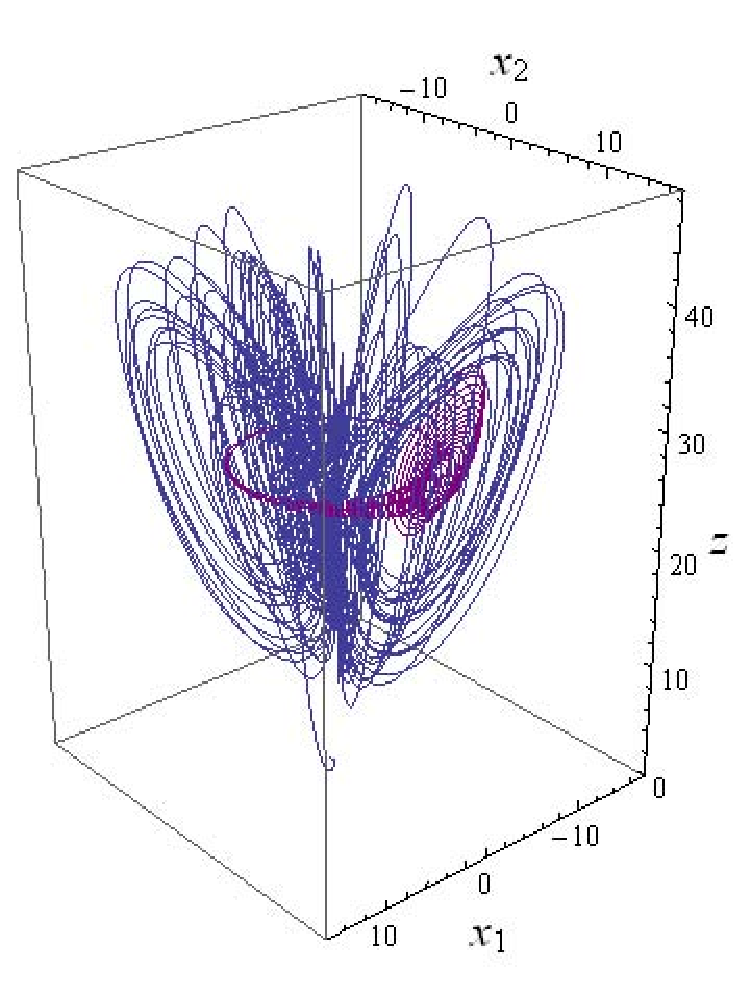
\includegraphics[width=0.35\textwidth]{CLEx1x2zRelEqu}
\end{center}
\caption{
Cartesian $\{x_1,x_2,z\}$ plot of the \cLf\ (a) with initial point
close to $\REQB{1}$, (b) superimposed over the strange attractor of
\reffig{fig:CLEx1x2z}.
    }
\label{fig:CLERelEqui}
\end{figure}
%%%%%%%%%%%%%%%%%%%%%%%%%%%%%%%%%%%%%%%%%%%%%%%%%%%%%%%

As discussed above, there are in total eight relative
equilibria. \refFig{fig:FourRelEquil} shows the flow with
initial point at four of these eight points and plotted in
Cartesian coordinates. Each of the initial points lies on the
circle. As the flow itself is rotationally invariant, all
of these eight relative equilibria are equivalent. From
here on, we only examine the properties of the point defined
above as $\ssp_{\REQB{}1}$.

%%%%%%%%%%%%%%%%%%%%%%%%%%%%%%%%%%%%%%%%%%%%
% computed by equilibrium.nb
\SFIG{ProblemsPill} %FourRelEquil}
{}{
Plot of four different relative equilibrium solutions (red,
yellow, green, blue). Some of the plots almost exactly
overlap and are not easily distinguishable.
}
{fig:FourRelEquil}
%%%%%%%%%%%%%%%%%%%%%%%%%%%%%%%%%%%%%%%%%%%%

\subsection{Eigen-system of the polar \stabmat}
As in \refsect{sect:stability}, we now find and plot the eigensystem of the stability matrix in order to understand the stability of $\REQB{1}$. Using the same methods described there, we find the eigenvalues
\[
(\lambda_{1,2},\lambda_3,\lambda_4)
= (0.0938179 \pm 10.1945 i,-11.0009,-13.8534)
\]
with the eigenvectors
\bea
\Re e_{1} &=& \Re e_{2} = (-0.266121, -0.0321133, 0.00034139, 0.719222)
\continue
\Im e_{1}  &=& -\Im e_{2} = (-0.295017, 0.569063, -0.000551886,0)
\continue
e_3 &=& (-0.0883591, -0.0851485, -0.989135, -0.0809553)
\continue
e_4 &=& (-0.855586, -0.329912, -0.00273531, -0.398902)
\,.
\label{eigVecQ1}
\eea

As in \refsect{sect:stability}, we can also plot the flow
(in polar coordinates) with an initial point very near to
$\REQB{1}$ along one of the eigenvectors.
\refFig{fig:CLEQ1} shows just this.
%%%%%%%%%%%%%%%%%%%%%%%%%%%%%%%%%%%%%%%%%%%%%%%%%%%%
% computed by eigensystem.nb
\begin{figure}[h]
\begin{center}
(a) %~\includegraphics[width=0.42\textwidth]{CLEQ1}
(b) %~\includegraphics[width=0.28\textwidth]{CLEQ1t100}
\end{center}
\caption{
(a) $\{\rho_1, \rho_2, z\}$ plot of the eigenvector $e_3$
(black) and the polar \cLf\ at initial values of
$\frac{1}{100}, \frac{2}{100}, \frac{3}{100}, \frac{4}{100},
\frac{5}{100},$ and $ \frac{6}{100}$ of $e_3$ (red, orange,
yellow, green, blue, violet) with $t$ from 0 to
$2\,\period{spiral}=1.232\cdots$, (b)
with initial point at $ \frac{6}{100} e_3$ (violet) and with
$t$ from 0 to 100.
    }
\label{fig:CLEQ1}
\end{figure}
%%%%%%%%%%%%%%%%%%%%%%%%%%%%%%%%%%%%%%%%%%%%%%%%%%%%%
                                                    \exerbox{exer:EigenQ1}
                                                    \exerbox{exer:PlotPolEigenQ1}

\section{\Reducedsp}
\label{sect:reducedStateSp}

Finally, we move on to the goal of the project, reducing the
state-space of the \cLe\ to only four dimensions. We present
two different versions of the `method of moving frames.' The
method can introduce singularities of the type we have
encountered in the polar coordinate reformulation, as in
\reffig{fig:PCsimulPolar}. We encounter these in applying
`polar' version of the method, but not in the other, more
general version. We finish by reproducing Siminos
`integration on the \csection' which - inspite of lacking a
theoretical justification - projects the \cLf\ to a nice
Lorenz-type attractor.

This section of the report is written in collaboration with
E.~Siminos and P.~Cvitanovi\'c.

\subsection{Method of moving frames, finite time steps}
\label{sect:MovFrame}

     \Private{
\noindent{\bf Predrag -
July 19, Aug 12 2009}: %\\
    }

Siminos\rf{SiminosThesis} discusses symmetry reduction by the
method of {\em moving frames} of Cartan\rf{CartanMF}, in the
formulation of Fels and
Olver\rf{FelsOlver98,FelsOlver99,OlverInv}.
                                                \exerbox{exer:SO2cSect}
The moving frames method allows the determination of (in
general non-polynomial) invariants of the group action by a
simple and efficient algorithm that, as argued in
\rf{SiminosThesis}, works well in high-dimensional \statesp s.
    \PC{Vaggelis, add references here? {\bf ES}: mmm...
SiminosThesis?} \PC{Vaggelis, why ``(non-polynomial)''
invariants? length$^2$ is polynomial {\bf ES}: In general we
don't get invariant polynomials 	from the moving frame
method applied to high dimensional representations of compact
Lie groups. 	For CLe we get a polynomial invariant and two
invariants that are rational functions of polynomials.
     }

Split up the integration of the $\SOn{2}$-equivariant ODE into
a sequence of short time steps, each followed by a rotation
such that the next segment initial point is in the point
$\ssp^{*}$ {\slice}, a $(d\!-\!1)$-dimensional hyperplane
normal to the group rotation tangent $t^{*}$ at point
$\ssp^{*}$:
\beq
(\ssp- \ssp^{*}) \cdot t^{*}=0
    \,,\qquad
t^{*} = \Lg \cdot \ssp^{*}
\,.
\ee{PCsectQ}
For any $\hat{\ssp}$, $\ssp =
\mathbb{G}(\theta)\cdot\hat{\ssp}$ is defined to be the
rotation of $\hat{\ssp}$ that lies in the \slice. Such a
map from a point in space to the group action is called a
\emph{moving frame} in the formulation of Fels and
Olver\rf{FelsOlver98,FelsOlver99,OlverInv}. A generic point
$\ssp^{*}$ not on the $z$ axis should suffice to fix a good
\slice, for example a point on an \reqv\ group orbit,
$\ssp^{*} = \ssp_{\REQB{}1}$.
                                                    \exerbox{exer:PCsectionCLe}
As $\ssp^{*} \cdot t^{*}=0$ by the antisymmetry of
$\Lg$, \refeq{PCsectQ} reduces to the condition
\beq
0 = \ssp \cdot \Lg \cdot \ssp^{*}
  %= \mathbb{G}(\theta) \cdot \hat{\ssp}   \cdot \Lg \cdot \ssp^{*}
	=\hat{\ssp} \cdot \mathbb{G}(\theta)^T \cdot \Lg \cdot \ssp^{*}
\ee{PCsectQ1}
that determines $\theta$ for a given $\hat{\ssp}$. Each
circle intersects the section exactly twice,  so there are
two solutions, separated by $\pi$. We select the one
with a smaller clockwise rotation angle into the \slice.
The $z$-axis invariant subspace is always within the section,
so this is a nice, globally transverse \slice.

%%%%%%%%%%%%%%%%%%%%%%%%%%%%%%%%%%%%%%%%%%%%%%%%%%
% computed by PCunrot.nb
\SFIG{ProblemsPill} %PCunrot}
{}{
Method of moving frames, finite time steps version: a
trajectory started on the \slice, with $\ssp_1^{(0)}
=0$, evolves for a finite time to a \statesp\ point with a
non-zero $\hat{\ssp}_1^{(1)}$. The {\em entire} \statesp\ is then
rotated (the `frame is moved') so that the equivalent point
on the circle lies on the \slice, $\ssp_1^{(1)} =0$.
Thus after every finite time step followed by a rotation the
trajectory returns to the 4$\dmn$ $\ssp_1 =0$
\reducedsp.
}
{fig:PCunrot}
%%%%%%%%%%%%%%%%%%%%%%%%%%%%%%%%%%%%%%%%%%%%%%%%%%

\refFig{fig:PCunrot} illustrates the method of moving frames,
finite time version, for a \slice\ motivated by the polar
form of the \cLe\ of \refsect{sect:coordChange}. It is
defined, for example, by taking
$(x^{*}_1,x^{*}_2,y_1^{*},y_2^{*})=(0,1,0,0)$,
$x_1=0,\,x_2>0$. Start at $\ssp^{(0)}$ with $\ssp_1^{(0)}
=0$, evolve for a finite time to $\hat{\ssp}^{(1)}$. Compute
the polar angle $\theta_1$ of $\hat{\ssp}^{(1)}_1$ in the
$(\ssp_1,\ssp_2)$ plane, and rotate the {\em entire}
\statesp\ (hence `moving frame') clockwise by $\theta_1$,
$\ssp^{(1)} = \mathbb{G}(\theta_1) \cdot \hat{\ssp}^{(1)}$,
to satisfy the $\ssp_1=0$ \slice\ condition. Repeat. The
trajectory remains in the 4$\dmn$ $\ssp_1=0$
\reducedsp.
    \PC{complete \refFig{fig:PCunrot}
        - need to draw a longer segment of the initial trajectory,
        to make it clearer that the whole segment is rotated.
       }

\subsection{Method of moving frames, differential formulation}
\label{sect:MovFrameODE}


\begin{bartlett}
I made a wrong mistake.
\bauthor{Yogi Berra}
\end{bartlett}

     \Private{
\noindent{\bf Predrag, Vaggelis -
Aug 13 2009}: %\\
    }
%\noindent{\bf Vaggelis -
%August 12 2009}: %\\
%\refeq{EqMotionMovFramePC} is correct, there are problems with the derivation.
%PC Aug 13 2009: fixed the details as suggested

                                                    \exerbox{exer:CLEsmall-x1x2}
                                                    \exerbox{exer:csectionCLeODE}
                                                    \exerbox{exer:csectionPhase}
                                                    \exerbox{exer:SiminosSlice}
Infinitesimal time version of the moving frames symmetry
reduction is attained by taking small time steps in
\reffig{fig:PCunrot} and dropping the higher order terms, as
in \refsect{sect:SymmDyn}. For infinitesimal  $d\theta$ we
set $\sin d\theta \approx d\theta$, $\cos d\theta \approx
1$, $\mathbb{G}(d\theta) \approx {1}+ d\theta \, \Lg $, and
the condition \refeq{PCsectQ} for rotating an infinitesimal
time evolution step $dx = v\,dt$ back into the \slice\
\[
0 = (\ssp + dx) \cdot \mathbb{G}(d\theta)^T \cdot \Lg \cdot \ssp^{*}
  \approx (\ssp + dt\,v) \cdot (1+ d\theta\,\Lg)^T \cdot \Lg \cdot \ssp^{*}
  \approx dt\,v \cdot \Lg \cdot \ssp^{*} - d\theta\,\ssp \cdot \Lg \cdot \Lg \cdot \ssp^{*}
\]
%\ES{It is $\Lg^T=-\Lg$.}
yields
\beq
d\theta \approx \frac{v \cdot \Lg \cdot \ssp^{*}}
                     { \ssp \cdot \Lg \cdot \Lg \cdot \ssp^{*}} \,  dt
\,.
\ee{MFdtheta}

%%%%%%%%%%%%%%%%%%%%%%%%%%%%%%%%%%%%%%%%%%%%%%%%%%
% File: infMF.xfig
\SFIG{ProblemsPill} %infMF}
{}{
Method of moving frames, infinitesimal formulation.
}
{fig:infMF}
%%%%%%%%%%%%%%%%%%%%%%%%%%%%%%%%%%%%%%%%%%%%%%%%%%

Let $u(\ssp)$ be the vector field that generates the flow in
the \reducedsp. According to \reffig{fig:infMF}, in
the limit that $\mathbb{G}(d\theta) \approx 1+d\theta\,\Lg$ the
infinitesimal time step under $u$ is connected to the time
step under $v$ by
    \PC{in \reffig{fig:infMF}:\\
        * Change $R$ into $\mathbb{G}$. \\
        * Draw $z$ axis
        (would lie horizontal in the present version, so tilt the figure).\\
        * Indicate $d\theta$ by drawing from origin, spanned by arc $x, x+v dt$.\\
        * Include a segment of the group-orbit ellipse, so $t^{*}$ is
          clearly visualized as a tangent.\\
        * Add arrows to $v dt$, $u dt$.
        }
\[
 \ssp+u\,dt=  (1+d\theta\Lg)\cdot(\ssp+v dt)\,.
\]
Dropping second order terms, dividing through with $dt$
\[
 u = v+\frac{d\theta}{dt} \,\Lg\cdot\hat{x}
 \,,
\]
and substituting \refeq{MFdtheta} gives the \reducedsp\ equations:
\beq
\dot{\ssp} = v - \frac{(v \cdot \Lg \cdot \ssp^{*})}{(\ssp \cdot\ssp^{*})_4}
                 \, \Lg \cdot \ssp
\,,
\ee{EqMotionMovFramePC}
where we have used the fact that
$- \ssp \cdot \Lg\cdot\Lg \cdot \ssp^{*}
 = (\ssp \cdot \ssp^{*})_4 =
    x_1 x_1^{*}
   +x_2 x_2^{*}
   +y_1 y_1^{*}
   +y_2 y_2^{*}
$
is the dot-product restricted to the 4-dimensional
representation of $\SOn{2}$. By construction, the motion
stays in the $(d\!-\!1)$-dimensional \slice.
                                                        \exerbox{exer:csectionReduced}
    \PC{
A more elegant derivation is given in
\refrefs{rowley_reconstruction_2000,rowley_reduction_2003},
and will be incorporated in \refref{SiminosThesis} and a coming article on this
topic.
    }

A generic  $ \ssp^{*}$ can be brought to form $ \ssp^{*} =
(0,1,y_1^{*},y_2^{*})$ by a rotation and rescaling. Then $\Lg
\cdot \ssp^{*}  = (1,0,y_2^{*},-y_1^{*})$, and
\beq
\frac{(v \cdot \Lg \cdot \ssp^{*})}{(\ssp \cdot\ssp^{*})_4} =
\frac{v_1 + v_3 y^{*}_2 -v_4 y^{*}_1}
     {x_2 + y_1 y^{*}_1 + y_2 y^{*}_2}
%\frac{v_1 x^{*}_2 -v_2 x^{*}_1 + v_3 y^{*}_2 -v_4 y^{*}_1}
%     {v_1 x^{*}_1 + v_2 x^{*}_2 + v_3 y^{*}_1 + v_4 y^{*}_2}
\,.
\label{PCsectSin}
\eeq

%
%%%%%%%%%%%%%%%%%%%%%%%%%%%%%%%%%%%%%%%%%%%%%%%%%%%%%%%%%%%%%%%%%%
% CLEpcSect.png computed by  CLEfinal.nb (repo: vaggelis)
% CLEpcSect2.png computed by CLEfinal.nb (repo: vaggelis)
\begin{figure}[ht]
\begin{center}
(a) % 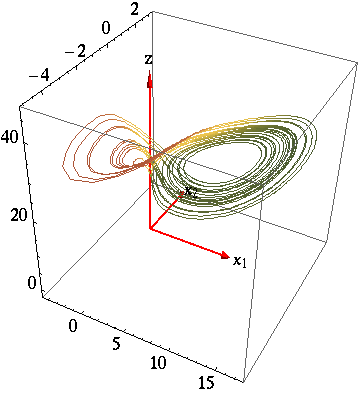
\includegraphics[width=0.40\textwidth]{CLEpcSect}
(b) %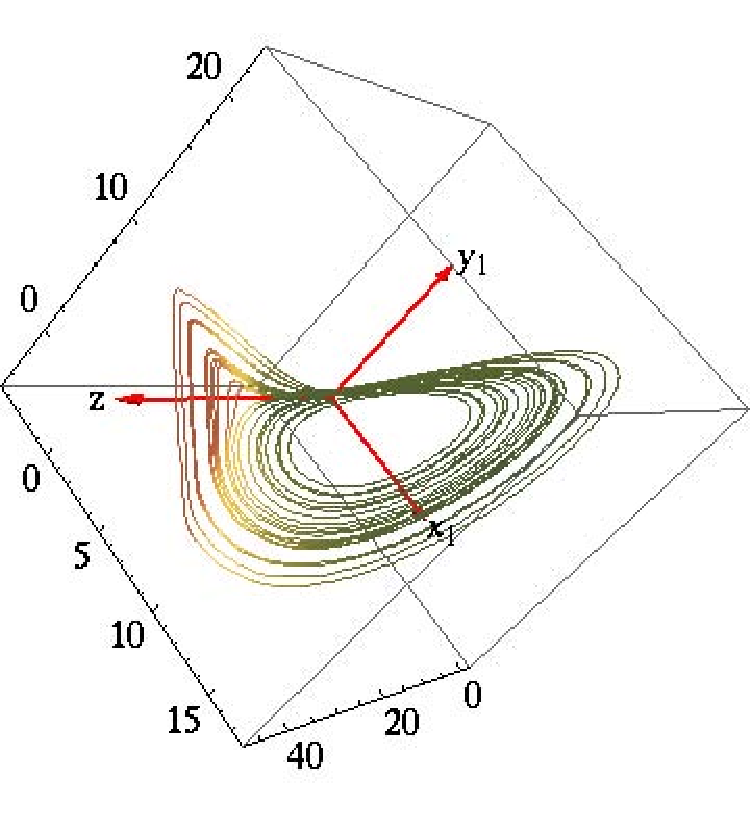
\includegraphics[width=0.43\textwidth]{CLEpcSect2}
\end{center}
\caption{
Method of moving frames, \slice\ fixed by a point on an
\reqv\ group orbit, $\ssp^{*} = \ssp_{\REQB{}1}$. The strange
attractor of \reffig{fig:CLEx1x2z} in the \reducedsp\
of \refeq{EqMotionMovFramePC}:
(a) $\{x_1,x_2,z\}$ projection,
(b) $\{x_1,y_1,z\}$ projection.
Color-coding indicates $(\hat{\ssp} \cdot \hat{\ssp^{*}})_4$
where $\hat{.}$ stands for unit vector, with green indicating values
of the inner product close to $1$ and brown indicating values
close to $0$.
    }
\label{fig:CLEpcSect}
\end{figure}
%%%%%%%%%%%%%%%%%%%%%%%%%%%%%%%%%%%%%%%%%%%%%%%%%%%%%%%%%%%%%%%%
%
A long time trajectory of \refeq{EqMotionMovFramePC} with
$x^*$ on the \reqv\ \REQB{1} group orbit is shown in
\reffig{fig:CLEpcSect}.
\ES{I will add a scale in \reffig{CLEpcSect} but it is too
late here to do it tonight.}
As initial condition
we chose an initial point on the unstable manifold
of \REQB{1}, rotated back to the \slice\ by angle $\theta$ as
prescribed by \refeq{PCsectQ1}. In \reffig{fig:CLEpcSect} we
show the part of the trajectory for $t\in\left[70,100\right]$.
The \reqv, now an equilibrium of the
\reducedsp\ dynamics, organizes the flow into a R\"ossler type
attractor. There appears to be no singularity in this
attractor although we can run into trouble with
\refeq{EqMotionMovFramePC} wherever the denominator in
\refeq{MFdtheta} vanishes, \ie, the direction of group
action on the point $\ssp$ is perpendicular to the direction
of group action on $\ssp^*$.
                                                        \exerbox{exer:PCsectionCLe}
    \PC{ in \reffig{fig:CLEpcSect}:\\
        * Mark $\ssp_{\REQB{}1}$ \\
        * Draw stable eigenvector of $\ssp_{\REQB{}1}$\\
        * State value of $\ssp_{\REQB{}1}$ somewhere
        }


%%%%%%%%%%%%%%%%%%%%%%%%%%%%%%%%%%%%%%%%%%%%%%%%%%
% computed by PCunrot.nb
\SFIG{ProblemsPill} %PCunrot1}
{}{
Method of moving frames, continuous time version, for the
polar coordinates motivated $x^{*}=(0,1,0,0)$,
$x_1=0,\;x_2>0$, \slice. The strange attractor of
\reffig{fig:CLEx1x2z} in the \reducedsp,
$\{x_2,y_2,z\}$ projection exhibits a discontinuity at
$x_2=0$.
}
{fig:PCunrot1}
%%%%%%%%%%%%%%%%%%%%%%%%%%%%%%%%%%%%%%%%%%%%%%%%%%

Indeed, the method appears to encounter singularities in
subsets of \statesp\rf{SiminosThesis}.
For example, the \reducedsp\ equations \refeq{PCsectSin}
for the polar coordinates inspired \slice\
$x^{*}=(0,1,0,0)$, $x_1=0,\;x_2>0$,
%this is illustrated by \reffig{fig:PCunrot}.
%$(\rho_1,\theta_1)$ are polar coordinates, $\rho_1 =
%\sqrt{\ssp_1^{ 2} + \ssp_2^{2}}$, see \refeq{eq:CartToPol},
are given by
                                                    \exerbox{exer:csectionCLe}
\beq
\dot{\ssp} = v - \frac{v_1}{\ssp_2} \Lg \cdot \ssp
\,.
\ee{EqMotionMovFrame}
A typical trajectory is shown in \reffig{fig:PCunrot1}.
The problem with defining the \slice\ by
\refeq{EqMotionMovFrame} is apparently that it fixes rotations
in the $(\ssp_1,\ssp_2)$ plane, not the full 4\dmn\ space.

\subsection{Integration on the \csection}

\RW{We never really talked too much about this, and I'm not
sure that I understand it all that well. This is mostly what
I figured out last night on my own. You may want to check it
for being...true. It was also very late when I wrote it, so
it may not be entirely comprehensible.
{\bf PC:} seems OK.}
Our second method of symmetry reduction Siminos
\rf{SiminosThesis} calls {\em integration on the
\csection\ (II)}. Here, we use the projection operator
\beq
\PperpOp_{ij}(\ssp^{*})=\delta_{ij}-
\frac{(\Lg \cdot \ssp^{*})_i (\Lg \cdot \ssp^{*})_j}{(\Lg \cdot \ssp^{*})^2}
\eeq
to remove any components of the \cLe\ that are tangent to the
rotation about the $z$-axis. Unlike the method of moving
frames where we continually rotate points back to the
{\slice}, in this method the components of integration are
tangent to the rotation only when crossing the hyperplane
fixed by $\ssp^{*}$. We define the new flow
$\frac{dx}{dt}=\PperpOp(x^{*}) v(x)$, following
Siminos\rf{SiminosThesis}, as
\beq
\dot x_{\perp} = v(x)-\mathbb{T}x^{*}
  \frac{\mathbb{T}x^{*}\cdot v(x)}{(\mathbb{T}x^{*})^{2}}
\label{eq:IntSlice}
\eeq\,
where $\Lg$ is the same as defined above and $x^{*}$ is an
arbitrary point defining the {\csection}.
\RW{I'm having a
problem understanding this equation, now that I look at it
closer, it doesn't quite match the method used in Mathematica
notebooks PCunrot.nb or my unrotate.nb. Unless I'm
misunderstanding something, the denominator doesn't quite
fit? Is this just a typo or am I very tired?
{\bf PC:} Tired. Never again write the report the last night of the
project, research cannot be crammed.}
This approach results in a nice 4-dimensional projection of
the \cLf,  as Siminos showed in
\reffig{fig:CLEtransvII}\,(a). Using \refeq{eq:IntSlice}, we
were able to reproduce this in \reffig{fig:CLEtransvII}\,(b).
However, as we were not able to establish a  theoretical
foundation for this projection, it remains only an
interesting visualization suggested by the method of moving
frames, not a viable method for symmetry reduction in its own
right.

%%%%%%%%%%%%%%%%%%%%%%%%%%%%%%%%%%%%%%%%%%%%%%%%%%%%%%%%%%%%%%%%%%
\begin{figure}[ht]
\begin{center}
(a) %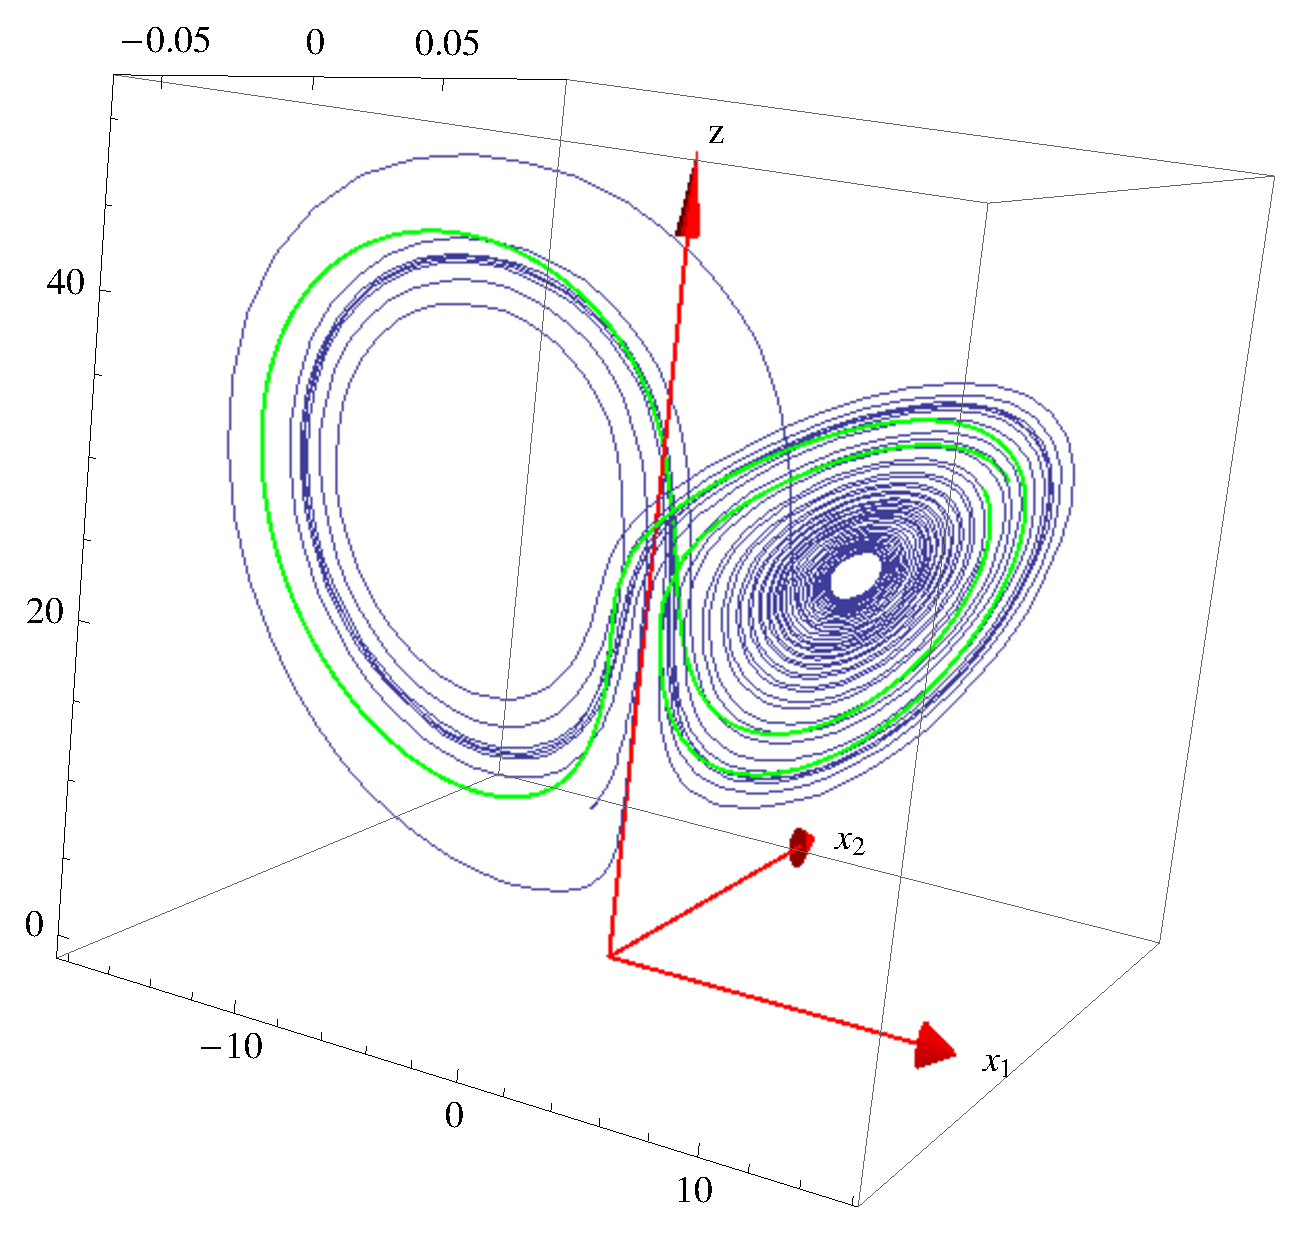
\includegraphics[width=0.45\textwidth, clip=true]{CLEtransvRPO}
(b) %\includegraphics[width=0.37\textwidth]{CLEUnrot2}
\end{center}
\caption[\CLe\ desymmetrization with transverse integration II]{
Restriction of \cLe\ dynamics on the {\slice} $\mathcal{K}$ through
\refeq{eq:difeqTransvII}. A trajectory initiated on the unstable
manifold of $\REQB{1}$ is shown in blue and \rpo\ ``011'' is shown
in green.
($e=1/10$, $\ImrCLor=0$).
(a) From Siminos Ph.D. thesis\rf{SiminosThesis}, (b) our
implementation.
    }
\label{fig:CLEtransvII}
\end{figure}
%%%%%%%%%%%%%%%%%%%%%%%%%%%%%%%%%%%%%%%%%%%%%%%%%%%%%%%%%%%%%%%%

\section{Conclusions}

Both the method of moving frames and integration on the
cross-section are still under development. We are not yet
sure whether either could be considered a success or failure.
The method of moving frames seems so far to produce a figure
without singularities, but it would require further work to
verify that singularities never occur. Integration on the
\csection\ also produces a smooth flow, resembling the
classical Lorenz attractor, and one could use the same tools
to analyze it. This method seems to work, although there is
no rigorous reason why it should.

Future work should investigate in more depth the viability of
the methods studied here. New methods (hopefully more
successful than the ones we have tested) with which to remove
the symmetry in the \cLe\ and multitude of other dynamical
systems with continuous symmetries need to be developed.
Siminos Ph.D. thesis\rf{SiminosThesis} addresses some of
these issues. In this project we have discussed, understood,
and tested the `moving frames' method as applied to \cLe\ in
the thesis. Much work still remains before these are viable
methods for higher-dimensional flows.

\section{Stability of \reqva}

\subsection{Hilbert polynomials}

The polynomials \refeq{eq:ipLaser} form a Hilbert basis for the \cLe.
\beq
\begin{split}
    u_1 &= x_1^2+x_2^2 \cont
    u_2 &= y_1^2+y_2^2 \cont
    u_3 &= x_1 y_2-x_2 y_1\cont
    u_4 &= x_1 y_1+x_2 y_2\cont
    u_5 &= z\,.
    \label{eq:ipLaser}
\end{split}
\eeq
In terms of the polar coordinates for the \cLe, these polynomials are
	\PC{shouldn't the first two be $\rho_1^2,\rho_2^2 $?}
\beq
\begin{split}
    u_1 &= \rho_1 \cont
    u_2 &= \rho_2 \cont
    u_3 &= - \rho_1 \rho_2 \sin \theta \cont
    u_4 &= \rho_1 \rho_2 \cos \theta \cont
    u_5 &= z\,.
    \label{eq:hilPolar}
\end{split}
\eeq
The \cLe\ in the Hilbert basis are:
\beq
\begin{split}
  \dot{u}_1 &=2\,\sigma\,(u_4-u_1)\,,\\
  \dot{u}_2 &=-2\left(\,u_2 - r_2\, u_3 -\,(r_1-u_5)\,u_4\right)\,,\\
  \dot{u}_3 &=-(\sigma\, +1)\,u_3+r_2\, u_1+e\, u_4\,,\\
  \dot{u}_4 &=-(\sigma\, +1)\,u_4+\,(r_1-u_5)\,u_1+\sigma\, u_2-e\,u_3\,,\\
  \dot{u}_5 &=u_4-b\, u_5\,.
\end{split}
\label{eq:CLEip}
\eeq
The relative equilibrium in polar coordinates is $\left( \rho_1 , \rho_2 , \theta , z \right) = \left(\sqrt{b \left(r_1 -d\right)},\sqrt{b d \left(r_1 -d\right)},\theta_Q, r_1 -d\right)$ where $d = 1+ \frac{e^2}{\left(\sigma +1 \right)^2}$ and $\theta_Q$ is the angle such that $\cos \theta_Q = \sqrt \frac{1}{d}$ and $\sin \theta_Q = -\sqrt \frac{d-1}{d}$.

So $\left( b \left(r_1 -d\right) , b d \left( r_1 -d \right) , b \left(r_1 -d\right) \sqrt{d-1}, b \left(r_1 -d\right), r_1 -d\right)$ is the relative equilibrium in this Hilbert basis.

\exercise{Hilbert basis singularities}{\label{exer:CLEipSyz}
% Predrag extracted from siminos/blog/CLEflotsam      Jun  5 2010
% also ChaosBook \example{Hilbert basis singularities}{\label{exam:CLEipSyz}
% 
When one takes syzygies into account in rewriting a
dynamical system, singularities are introduced. For instance,
eliminate $u_2$ using the syzygy, and show that you get
the reduced set of equations,
	\PC{I removed 
$  \dot{u}_2 = -2\left(\,\frac{u_3^2+u_4^2}{u_1} - \rho_2\, u_3
                -\,(\rho_1-u_5)\,u_4\right)
$
            }
\bea
  \dot{u}_1 &=& 2\,\sigma\,(u_4-u_1)
                \continue
  \dot{u}_3 &=& -(\sigma\, +1)\,u_3+\rho_2\, u_1+e\, u_4
                \continue
  \dot{u}_4 &=& -(\sigma\, +1)\,u_4+\,(\rho_1-u_5)\,u_1
                +\sigma\, {(u_3^2+u_4^2)}/{u_1}-e\,u_3
                \continue
  \dot{u}_5 &=& u_4-b\, u_5
\,,
\label{eq:CLEipSyz}
\eea
singular as $u_1\rightarrow 0$. (PC: check this - there might
be errors)
\authorES
    } %end \exer{Hilbert basis singularities}



The {\stabmat} in the Hilbert basis for the \cLe\ is
	\PC{This is [5$\times$5], but there are only 4 independent 
            variables. How does that show up in the eigensystem of
	    {\stabmat}?}
\beq
\begin{split}
\mathbb{A}=
\left(
\begin{array}{ccccc}
-2 \sigma & 0 & 0 & 2 \sigma & 0\\
0 & -2 & 2 r_2 & 2 \left(r_1 - u_5\right) & -2 u_4\\
r_2 & 0 & -\left(\sigma +1 \right) & e & 0\\
\left(r_1 -u_5 \right) & \sigma & -e & -\left(\sigma +1 \right) & -u_1\\
0 & 0 & 0 & 1 & -b
\end{array}
\right)
\end{split}
\eeq


\section{\Po s and dynamical averages}
\label{s:numerics}

\begin{figure}%[H]
\centering
(a)\!\!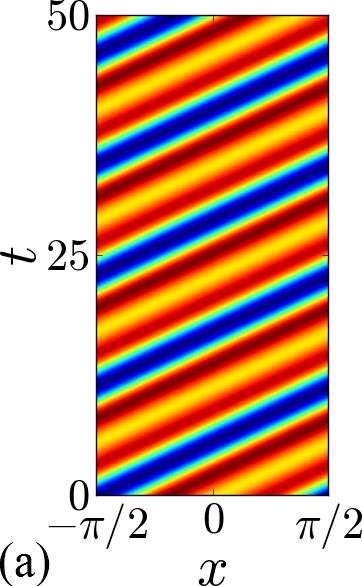
\includegraphics[width=0.22\textwidth]{2modes-conf-reqv}%
(b)\!\!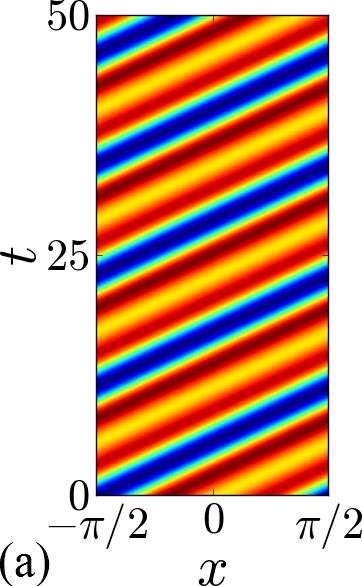
\includegraphics[width=0.22\textwidth]{2modes-conf-reqv}%
\caption{(Color online)
The \reqv\ \REQV{}{} in
 (a) the full \statesp, becomes an \eqv\ in
 (b) the symmetry-reduced configuration space.
}
\label{fig:2modes-conf-reqv}
\end{figure}

\begin{figure}%[H]
\centering
(a)\!\!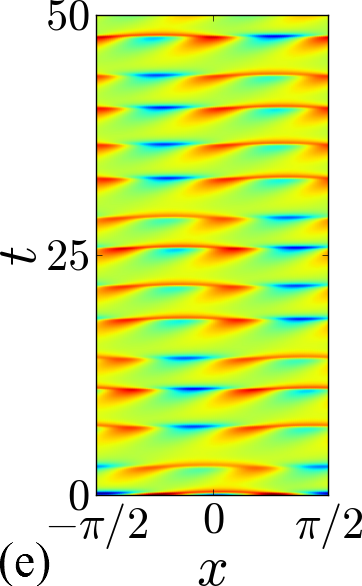
\includegraphics[width=0.22\textwidth]{2modes-conf-ergodic}
(b)\!\!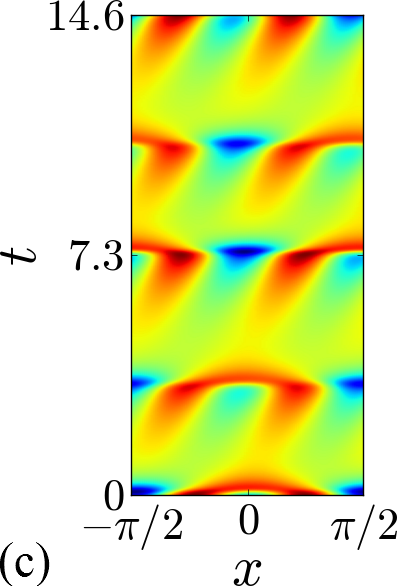
\includegraphics[width=0.22\textwidth]{2modes-conf-rpo}%
\caption{(Color online)
 (a) A typical ergodic trajectory of the \twomode\ system in the
 symmetry-reduced configuration space; clearly the unstable \reqv\
 \REQV{}{} in \reffig{fig:2modes-conf-reqv}\,(b) is far from a typical
 state.
 (b) Two repeats of \rpo\ \cycle{01}  (note the different time scale),
 in the symmetry-reduced configuration space. The dynamics is mostly
 dominated by the $m=1$ Fourier mode, interspersed by rapid shifts by
 $\approx \pm L/2$, dominated by the  $m=2$ Fourier mode.
}
\label{fig:2modes-conf}
\end{figure}

\begin{figure}%[H]
\centering
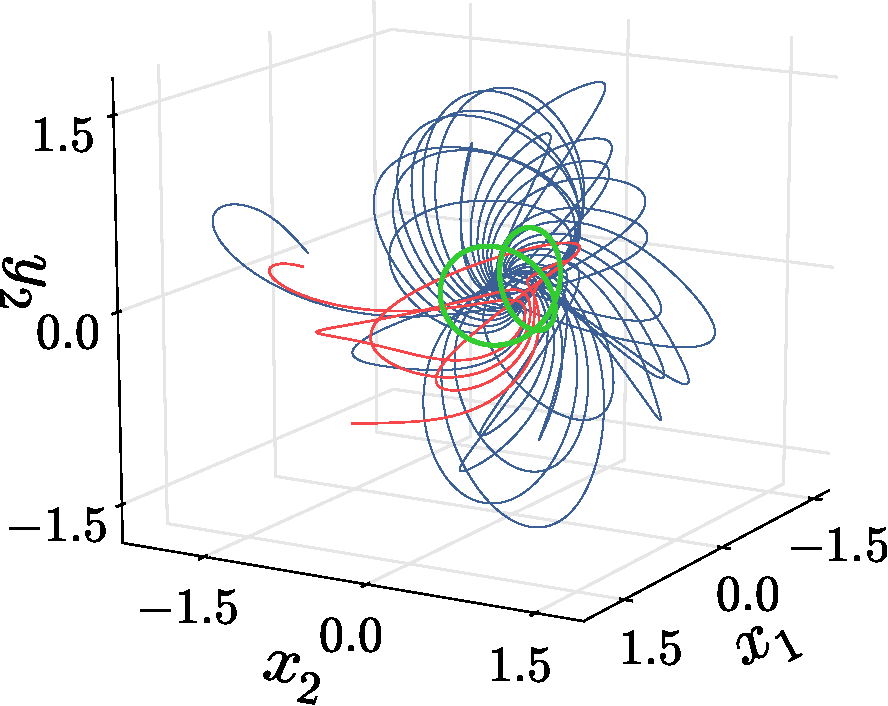
\includegraphics[width=0.45\textwidth]{2modes-ssp}
\caption{(Color online)
The same trajectories as in \reffig{fig:2modes-conf},
colored green, red and blue respectively,
in a 3D projection of the 4\dmn\ \statesp.
}
\label{fig:2modes-ssp}
\end{figure}

\begin{figure}%[H]
\centering
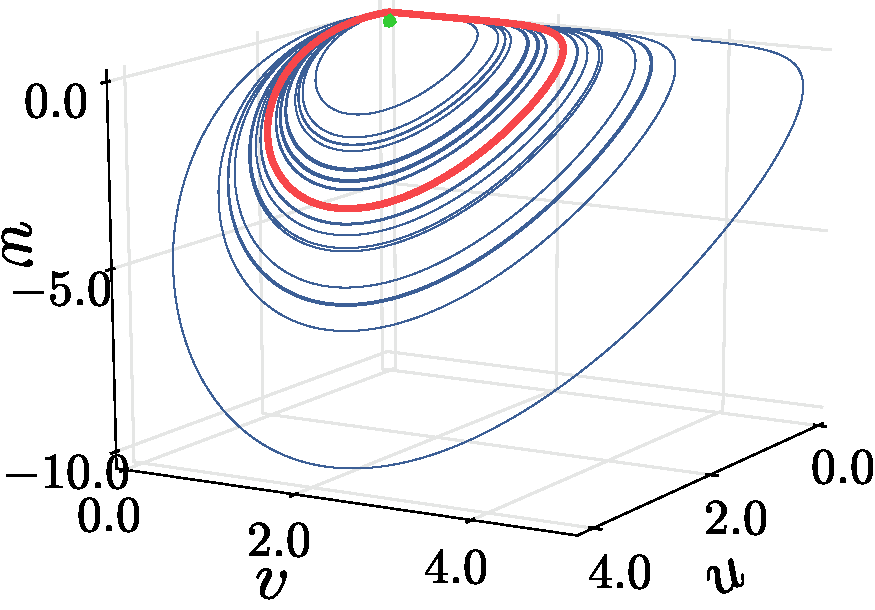
\includegraphics[width=0.45\textwidth]{2modes-invpol}
\caption{(Color online)
The same trajectories as in \reffig{fig:2modes-conf} and
\reffig{fig:2modes-conf-reqv}\,(a), colored green, red
and blue respectively, in a terms of 3 invariant polynomials.
The \reqv\ \REQV{}{} is now reduced to an \eqv, the green point.
}
\label{fig:2modes-invpol}
\end{figure}

\begin{figure}%[H]
\centering
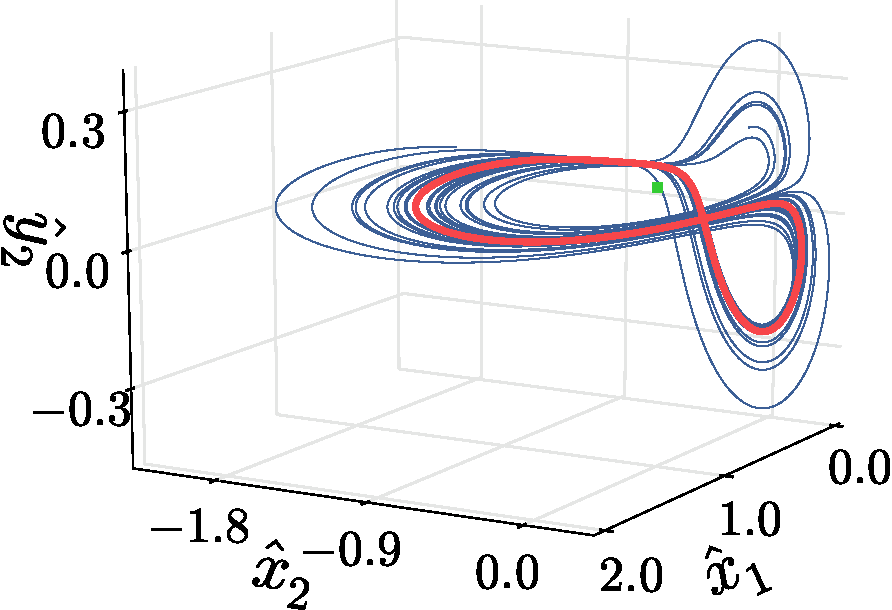
\includegraphics[width=0.45\textwidth]{2modes-sspRed}
\caption{(Color online)
The same trajectories as in \reffig{fig:2modes-conf} and
\reffig{fig:2modes-conf-reqv}\,(a), colored green, red
and blue respectively, in the 3\dmn\  first Fourier mode \slicePlane. The
\reqv\ \REQV{}{} is now reduced to an \eqv, the green point. In contrast
to the invariant polynomial representation \reffig{fig:2modes-invpol},
the qualitative difference between shifts by $\approx L/2$ and $\approx
-L/2$ in near passages to the {\sliceBord} is very clear, and it leads to
the unimodal Poincar\'e return map of \reffig{fig:psectandretmap}.
}
\label{2modes-sspRed}
\end{figure}

\PC{2014-07-14
Why $\pm L/2$ in \reffig{fig:2modes-conf} and
\reffig{fig:2modes-conf-reqv} and not $\pm \pi$?
}
\ES{2014-05-15}{I have replaced the second-mode slice, double-angled
figure in \reffig{2modes-conf-reqv}\,(b) with one resulting by integrating on the
$(0,0,1,0)$ slice, for consistency with panel (c). I hope Burak will
replace it with a publication quality figure of the same representation.
The trick of angle doubling will be introduced in its own section. }

To illustrate the \mslices\ on the \twomode\ system we choose a simple
set of parameters for which we observe interesting dynamics. These
parameters are listed in \refeq{eq:pars}. With this set of parameters,
we can write \twomode\ ODEs \refeq{eq:DangSO2} in terms of three parameters
$\{ \mu_1, c_2, a_2 \}$:
\bea
\label{eq:DangSO2set1}
  \sspC_1 &=& \mu_1 \,z_1 - z_1|z_1|^2 +c_1\,\overline{z}_1\,z_2
  \continue
  \sspC_1 &=& (1-\ii)\,{z_2}+a_2\,z_2|z_1|^2+\,z_1^2
\,,
\eea
Note that by setting $b_2 = 0$, we send the \reqv\ at $\invpol =
(0,-\mu_2/b_2,0,0)$ to infinity. Moreover, \refeq{PKinvEqs5a} yields
$\tilde{v} = (\mu_1 + \tilde{a}_1 \tilde{u})/(\mu_2 + \tilde{a}_2
\tilde{u} - \tilde{u} \tilde{b}_1)$. Substitution into \refeq{PKinvEqs5b}
allows one to solve for a single variable. By solving \refeq{PKinvEqs5}
with the parameter set \refeq{eq:pars}, we get two real roots, with
non-negative $u$ and $v$:
%the \eqva\ of the system in the invariant polynomial basis \refeq{Dang86(1.2)PK} as
\[
	\invpol_{\EQV{}} = (0,0,0,0)^T %\qquad \mbox{(double)}
\]
which is a double root and corresponds to an equilibrium of \refeq{eq:DangSO2}, and
\[
			 \invpol_{\REQV{}{}} = (0.193569,0.154131,-0.149539,-0.027178)^T\,,
\]
which is a {\reqv}. In real representation, a
representative point on  \REQV{}{} may be chosen as
\[
  \left(x_1, y_1, x_2, y_2\right) = \left(0.439966, 0, -0.386267, 0.070204\right)
\]
We visualize the dynamics of the \twomode\ system in four different
representations: 3D projections of the four-dimensional real valued
\statesp\ and invariant polynomials, in the 3D \slicePlane\ and on the 2D
configuration space plots on which the color-coded field $u(\conf,\zeit)$
is defined as follows:
\bea
	u(\conf, \tau) &=& \sum_{k=-2}^{2} \sspC_k(\zeit) e^{i k \conf}\, ,
	\continue && \mbox{where} \, \sspC_{-k} = \sspC_k^* \, \mbox{and} \,
	\sspC_0 = 0
\, .
\eea
\refFig{fig:2modes-conf}, \reffig{fig:2modes-conf-reqv}\,(a)
and \reffig{2modes-sspRed} show the sole \reqv\
\REQV{}{}, the \rpo\ \cycle{01}, and an ergodic trajectory of the
\twomode\ system in the four different representations discussed above.
Note that translation of the \reqv\ in the configuration space
\reffig{fig:2modes-conf-reqv}\,(a), corresponds to the \SOn{2} rotations in
the \statesp\ of Fourier modes in \reffig{2modes-ssp} (green curve) and
these orbits correspond to a single point in the symmetry reduced
representations of \reffig{fig:2modes-invpol} and \reffig{2modes-sspRed}.
Note also that the \rpo\ \cycle{01} translates/rotates as it advances in
configuration space (\reffig{fig:2modes-conf}\,(b)) and in the
equivariant \statesp\ \reffig{2modes-sspRed} (\reffig{2modes-ssp}),
whereas in the symmetry reduced plots (\reffig{fig:2modes-invpol} and
\reffig{2modes-sspRed}), it closes onto itself after one period.

\subsection{Finding cycles}

The simple structure of the symmetry reduced dynamics allows us to
determine the \rpo s of the \twomode\ system by means of a Poincar\'e
section and a return map. We illustrated this procedure in
\reffig{fig:psectandretmap}. Starting with an initial point close to the
\REQV{}{}, we computed a long ergodic trajectory of the symmetry reduced
\twomode\ system by integrating \refeq{e-so2red1stmode} (blue curve in
\reffig{fig:psectandretmap}\,{a)) and recorded its intersections (marked
with red in \reffig{fig:psectandretmap}\,{a)) with the Poincar\'e section
(transparent plane in \reffig{fig:psectandretmap}\,{a)), which includes
the \REQV{}{} and the imaginary part of its unstable stability
eigenvector (one of the green arrows in \reffig{fig:psectandretmap}\,{a)).
We then projected these intersections onto a basis $(v_1, v_2)$, which
spans the Poincar\'e section, and fit cubic splines to this set of
points, see \reffig{fig:psectandretmap}\,{b). The return map of arclengths
from the origin which is set to \REQV{}{} in
\reffig{fig:psectandretmap}\,{b), is unimodal with an sharp cusp located at its critical point, shown
in \reffig{fig:psectandretmap}\,{c). Note that the region corresponds to
the neighborhood of the \reqv\ $s = (0, 0.6)$ is never visited once the
flow leaves it and falls onto the chaotic attractor. For this reason, we
re-drew this return map after discarding the data corresponding to the
initial transients in \reffig{fig:psectandretmap}\,{d). We use this return
map to determine the accessible \rpo s  with their respective binary
symbol sequences.

\begin{figure}
\centering
  (a) 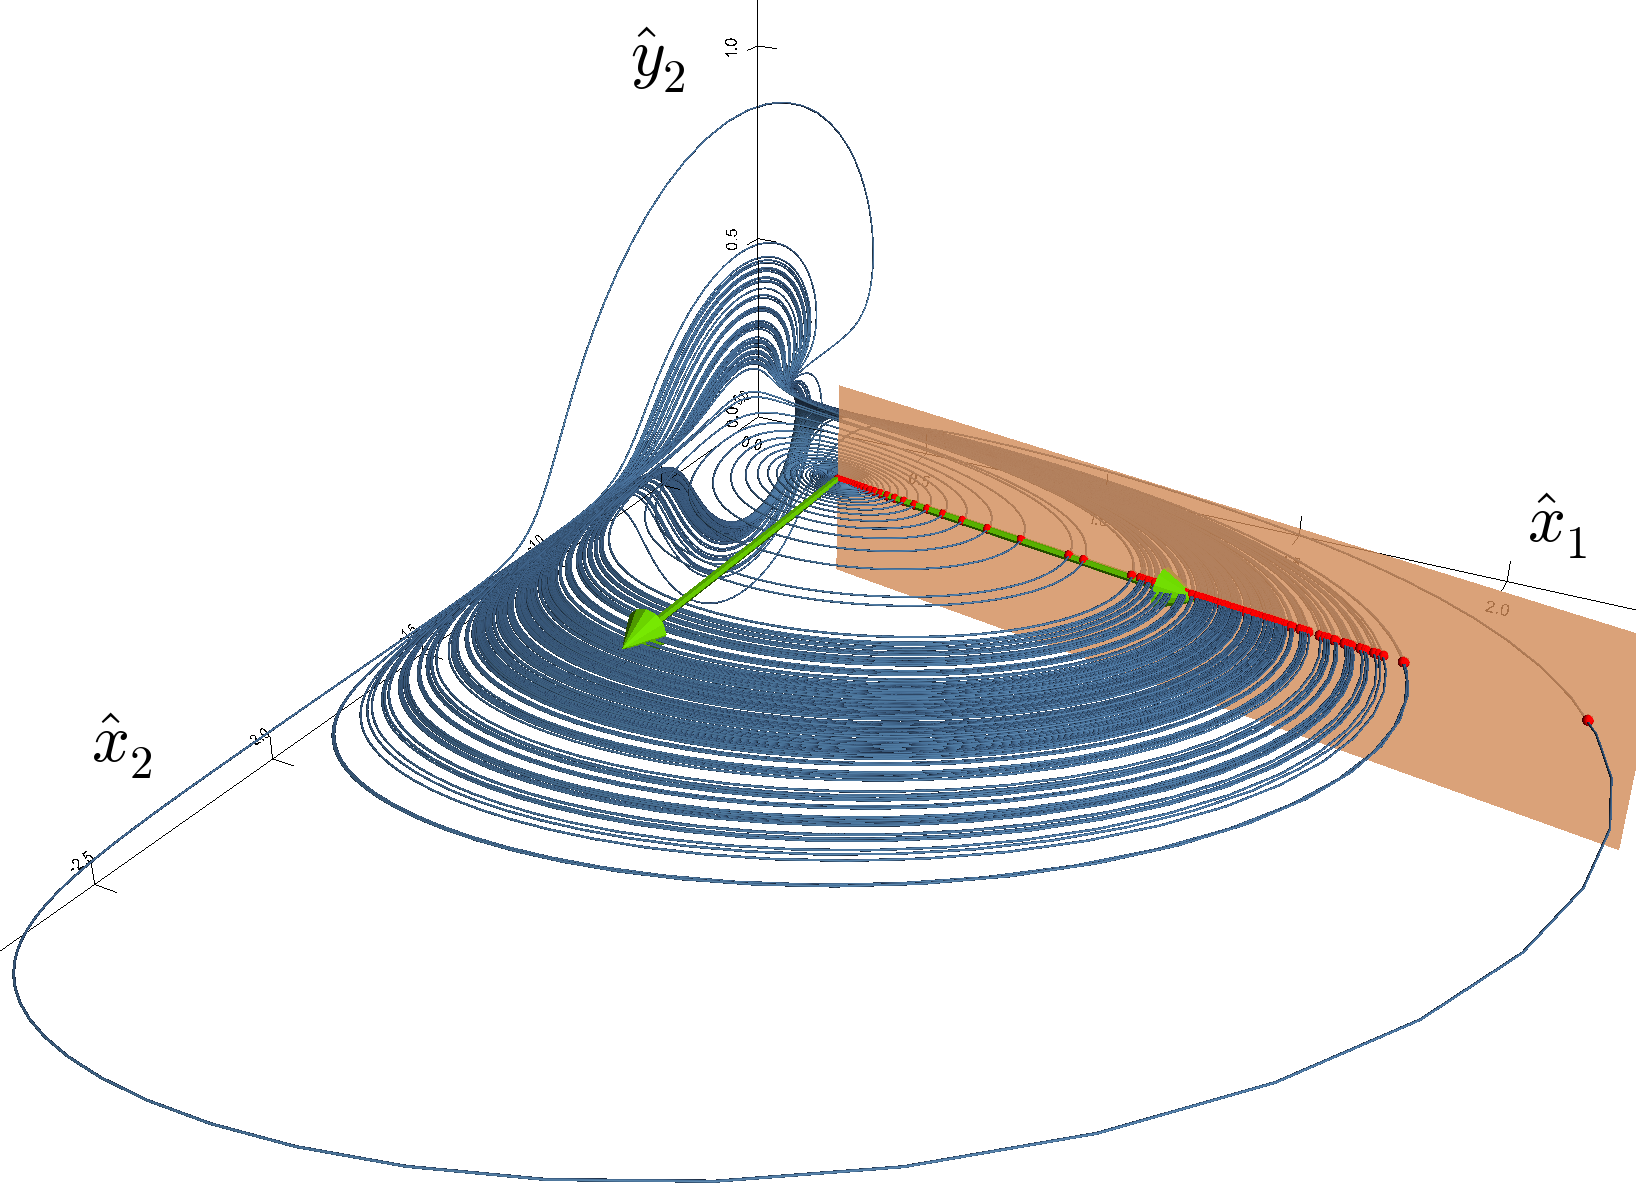
\includegraphics[width=0.45\textwidth]{BBpsecthd} \\
  (b) 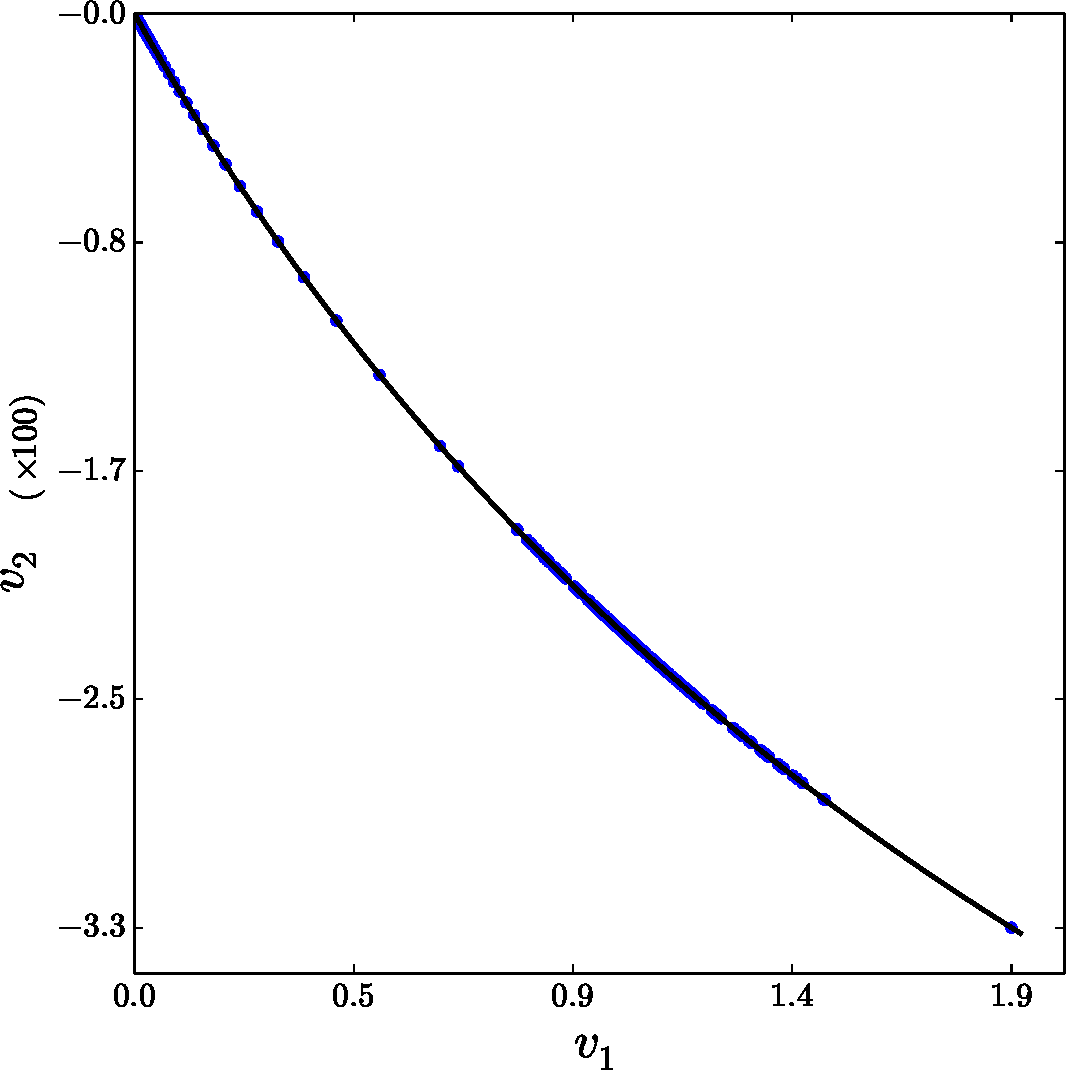
\includegraphics[width=0.20\textwidth]{BBpsectonslice}
  (c) 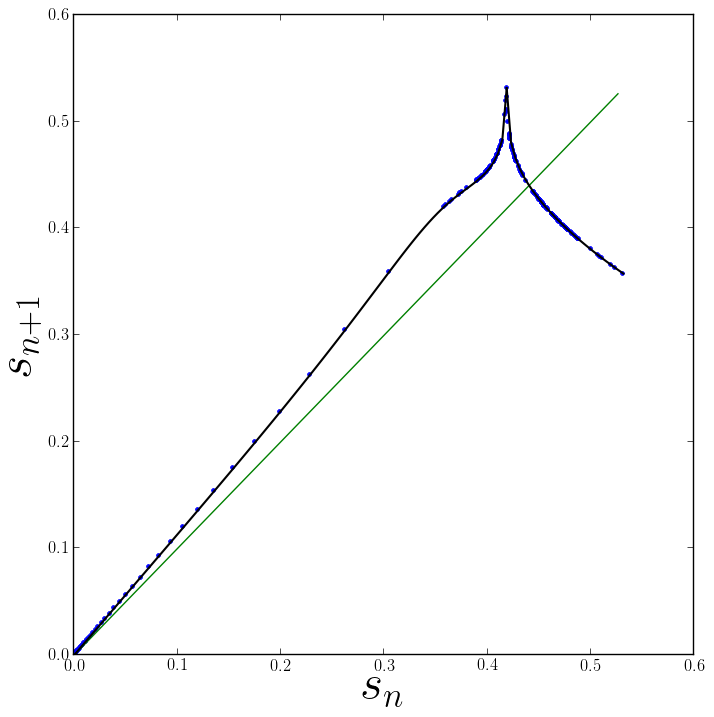
\includegraphics[width=0.20\textwidth]{BBretmaponslice} \\
  (d) 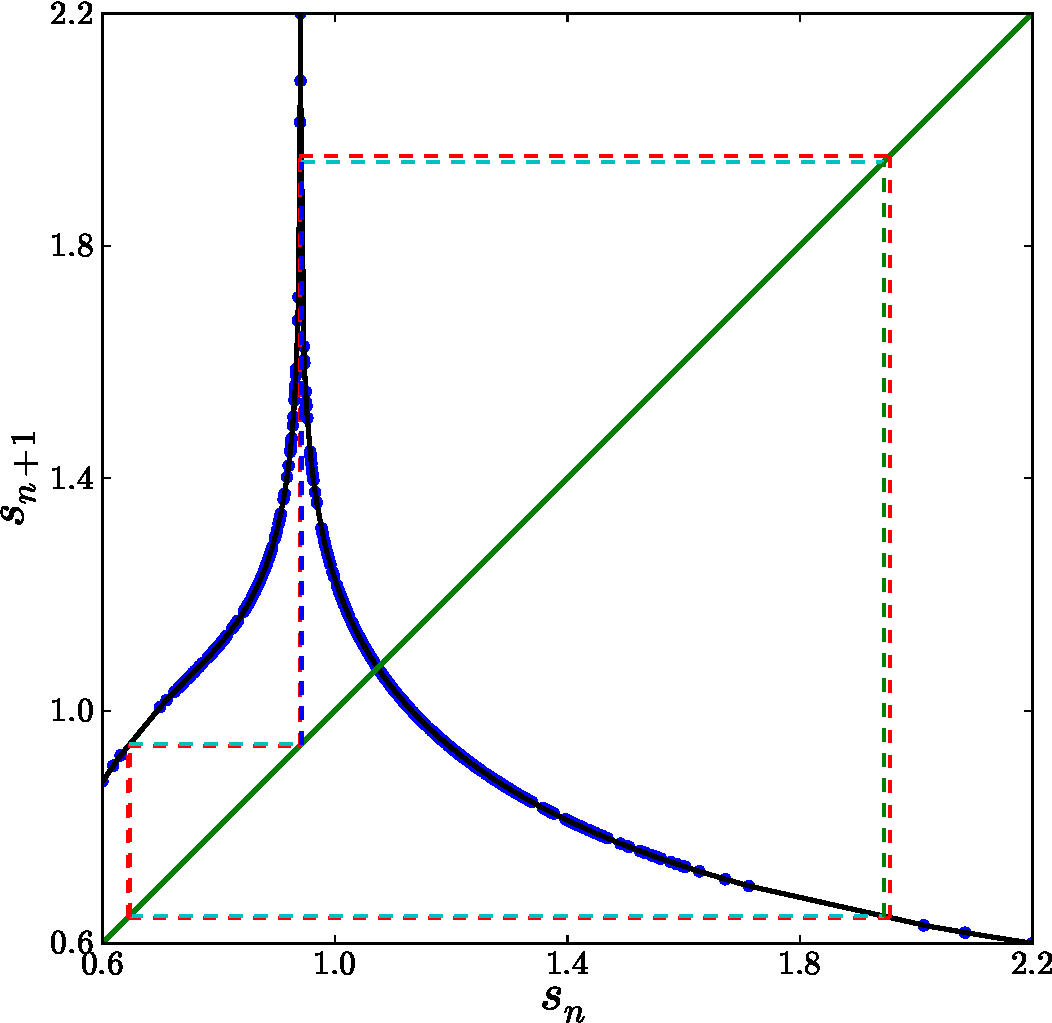
\includegraphics[width=0.45\textwidth]{BBretmaponsliceZoom}
\caption{(a) Symmetry reduced flow within the slice hyperplane (blue).
			Green arrows show the real and imaginary part of the unstable stability
			eigenvector $v_u$ of \REQV{}{}. A Poincar\'e section which includes
			$Im[v_u]$ is visualized as a transparent plane, and sections
			of the flow by the Poincar\'e section are marked with red.
		 (b) The Poincar\'e section which includes the \REQV{}{} and $v_u$ projected
			on to the basis within the plane shown in (a). Included is a
            transient trajectory initiated close to \REQV{}{}. Note that
		  	the vertical axis is magnified by $100$.
		 (c) The Poincar\'e arclength return map for the
		    Poincar\'e section (b).
		 (d) The return map without the transient points, framed by
            orbit of the critical point.
		 	Dashed lines show the 3-cycles \cycle{001} (red) and \cycle{011} (cyan).}
\label{fig:psectandretmap}
\end{figure}

Unimodal return map of \reffig{fig:psectandretmap}\,(d) lets us name the
periodic orbits of the \twomode\ system according to their binary
symbolic dynamics. Critical point of this map is at $s_C=0.98102264$,
corresponding to the tip of the return map. Topological coordinate of the
critical point, the kneading value, lets us determine the all admissible
cycles of the system. For a detailed introduction to the symbolic
dyanmics techniques we refer to \refref{DasBuch}. After determining the
admissible cycles, we find candidates corresponding to the admissible
symbol sequences from the return map, and feed them into a multiple
shooting Newton solver (see Appendix \ref{s:newton}) to precisely
determine the \rpo s. This way, we found the admissible cycles of the
\twomode\ system upto the topological length 12. In
\reffig{f-2modesrpofirst4} we show shortest $4$ of the \rpo s of the
\twomode\ system within the first Fourier mode \slicePlane . As seen from
\reffig{f-2modesrpofirst4}, trajectories of \cycle{001} and \cycle{011}
almost overlap in a large region of the \statesp . This behavior is also
manifested in the return map of \reffig{fig:psectandretmap}\,{d), where
we have shown cycles \cycle{001} and \cycle{011} with red and cyan
respectively. This is a general property of the \twomode\ cycles with odd
topological lengths: They come in pairs with almost equal Floquet
exponents, see \reffig{f-2modes-lambdaDist}.

\begin{figure}%[H]
\centering
 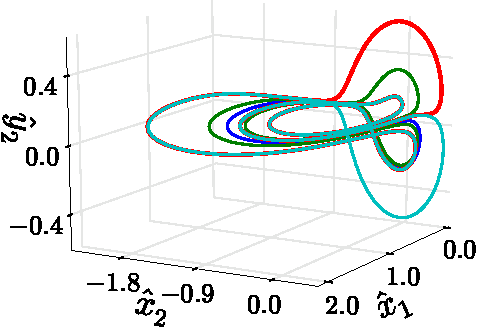
\includegraphics[width=0.45\textwidth]{2modesrpofirst4}
\caption{Shortest four \rpo s of the \twomode\ system: \cycle{1} (dark blue), \cycle{01} (green), \cycle{001} (red), \cycle{011} (cyan). Note that \rpo s \cycle{001} and \cycle{011} almost overlap everywhere except $\hat{x}_1 \approx 0$ .}
\label{f-2modesrpofirst4}
\end{figure}

\subsection{\CycForm s}
\label{s:DynAvers}

Spectrum of an observable, such as phase drift, or energy dissipation, of
a dynamical system is dual to the spectrum of its periodic orbits by
means of the classical trace formula\rf{DasBuch}
\beq
\sum_{\alpha=0}^{\infty} \frac{1}{s-s_{\alpha}} = \sum_p T_p \sum_{r=1}^{\infty} \frac{e^{r(\beta A_p - s T_p)}}{\oneMinJ{r}} .
\ee{e-ClassicalTraceFormula}

\begin{figure}%[H]
\centering
 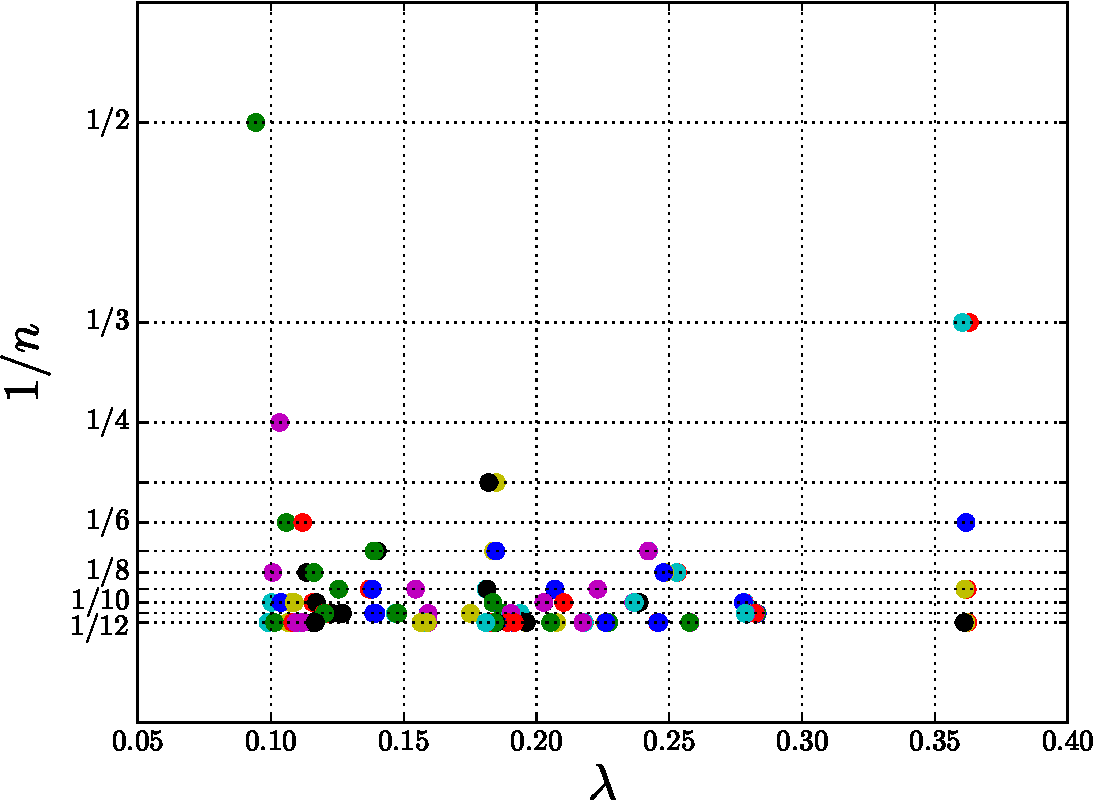
\includegraphics[width=0.45\textwidth]{2modes-lambdaDist}
\caption{Distribution of the leading Floquet exponents of \twomode\ cycles.}
\label{f-2modes-lambdaDist}
\end{figure}


Here, $s_{\alpha}$ are the eigenvalues of $\mathcal{A}$, the semigroup generator of the dynamical evolution of the observable $A$, outer sum on the RHS runs over the ``prime cycles'' of the system, $T_p$ is the period of the prime cycle $p$, $A_p$ is the value of the observable along the prime cycle, $\monodromy_p$ is the transverse (no marginal directions) monodromy matrix and $s$ and $\beta$ are auxilliary variables dual to the observable $A$ and time respectively.

While the classical trace formula \refeq{e-ClassicalTraceFormula} manifests the essential duality between the spectrum of an observable and that of the periodic orbits, in practice, it is hard to work with since the eigenvalues are located at the poles of
\refeq{e-ClassicalTraceFormula}. For this reason, one expresses this duality equivalently as the following spectral determinant
\beq
    \det (s-\mathcal{A}) = \exp \left( - \sum_p \sum_{r=1}^{\infty}
                             \frac{1}{r} \frac{e^{r(\beta A_p - s T_p)}}{\oneMinJ{r}} \right)\, ,
\ee{e-SpectralDeterminant}
logarithmic derivative of which gives \refeq{e-ClassicalTraceFormula}. The spectral determinant \refeq{e-SpectralDeterminant} is easier to work with since the spectrum of $\mathcal{A}$, is now located at the zeros of \refeq{e-SpectralDeterminant}. Convergence of \refeq{e-SpectralDeterminant} is still not obvious. More insight is gained by approximating $\oneMinJ{r}$ by the product of expanding Floquet multipliers and then computing the $r$ sum in \refeq{e-SpectralDeterminant}.
\bea
\oneMinJ{} &=& | (1 - \ExpaEig_{e,1})(1 - \ExpaEig_{e,2})... \continue
			&&(1 - \ExpaEig_{c,1}) (1 - \ExpaEig_{c,2}) ... | \nonumber \\
			&\approx& \prod_e |\ExpaEig_e| = |\ExpaEig_p|,
\eea
where $|\ExpaEig_{e,i}| > 1$ and $|\ExpaEig_{c,i}| < 1$ are expanding and contracting Floquet multipliers respectively. After this approximation, $r$-sum in \refeq{e-SpectralDeterminant} becomes the Taylor expansion of natural logarithm and it can be compactly written as follows:
\beq
1 / \zeta = \prod_r (1 - t_p) \, \mbox{where}, \, t_p = \frac{1}{|\ExpaEig_p|} e^{\beta A_p - s T_p} z^{n_p} .
\ee{e-DynamicalZeta}
Where we inserted the `order tracking' term $z$. For complete binary symbolic dynamics, the dynamical zeta function \refeq{e-DynamicalZeta} can be brought into the `curvature expansion' form:
\bea
1 / \zeta &=& 1 - t_0 - t_1 - (t_{01} - t_0 t_1 )  \label{e-CycleExpansion} \\
		  && - [(t_{011} - t_{01}t_1) + (t_{001} - t_{01} t_0)] - ... \continue
		  &=& 1 - \sum_f t_f - \sum_n \hat{c}_n \label{e-CurvatureExpansion}.
\eea
In the curvature expansion \refeq{e-CurvatureExpansion}, we grouped the contributions to the dynamical zeta function as `fundamental' contributions $t_f$ and `curvature' corrections. One expects the curvature corrections to be small since the longer prime cycles are `shadowed' by the combination of the shorter ones, the `pseudocycles'.

For complete binary symbolic dynamics, the only fundamental contributions to the dynamical zeta function are the cycles with topological length $1$, see \refeq{e-CurvatureExpansion}. This is not the case for any map since in general there might be non-trivial pruning rules, hence longer cycles can appear unshadowed. The Poincar\'e return map of \reffig{fig:psectandretmap}\,{d) is such a map with non-trivial pruning rules, however, note that cycles \cycle{001} and \cycle{011} passes very close to the tip of the cusp, the critical point, in \reffig{fig:psectandretmap}\,{d). This observation motivates us to approximate the return map of \reffig{fig:psectandretmap}\,{d), as if its tip is located at $s = 0.97986453$, where the cycle \cycle{001} lands, and omit the contributions above this point. We will refer this approximation as the `finite grammar approximation' since by doing it, we obtain single pruning rule; that is the symbol sequence $00$ is not allowed. This grammar is known as the `golden mean' pruning and a complete binary symbolic dynamics can be converted to the golden mean symbolic dynamics by substitution $0 \rightarrow 01$. We can write the dynamical zeta function for the golden mean pruned symbolic dynamics by replacing $0$s in \refeq{e-CycleExpansion} by $01$:
\bea
1 / \zeta &=& 1 - t_{01} - t_1 - (t_{011} - t_{01} t_1 ) \label{e-GoldenMeanCycleExpansion}\\
		  && - [(t_{0111} - t_{011}t_1) + (t_{01011} - t_{01} t_{011} ) ] - ... \nonumber
\eea
Note that all the contributions longer than topological length $2$ to the golden mean dynamical zeta function are in form of shadowing combinations. However, as we shall see, they are not small.

While dynamical zeta functions are useful for investigating the convergence properties, they are not exact, and their computational cost is same with that of the exact spectral determinants. For this reason, we will expand the spectral determinant \refeq{e-SpectralDeterminant} ordered in the topological length of cycles and pseudocycles as follows:
\beq
    \det (s-\mathcal{A}) =   \prod_p \exp \left( - \sum_{r=1}^{n_p r < N}
                             \frac{1}{r} \frac{e^{r(\beta A_p - s T_p)}
                                          }{\oneMinJ{r}} z^{n_p r} \right) \, .
\ee{e-SpectralDeterminantExp}
This is the form that we use to compute the spectral determinant. For each prime cycle, we compute the sum term in \refeq{e-SpectralDeterminantExp} truncated at the expansion order $N$, and then expand the exponential upto order $N$, and multiply this expansion with the contributions from previous cycles and drop terms with order greater than $N$. This way, we obtain the $N^{th}$ order spectral determinant \refeq{e-SpectralDeterminant}. Let us denote the resultant series after setting $z=1$ as
\beq
    F_N(s, \beta ) = 1 - \sum_{n=1}^{N} Q_n(s, \beta ) \, .
    \label{e-NthOrderSpectDet}
\eeq
Leading $0$ of $F_N(s, 0)$, $s_0$, corresponds to the leading eigenvalue of the Perron-Forbenius operator, $\gamma_0 = - s_0$, which can be interpreted as the `escape rate'. We expect the escape rate to be small, ideally zero, if the cycle expansion is good.
After finding $s_0$, we can compute the dynamical averages as follows:
Mean period:
\bea
    \langle T \rangle_N &=& \left. \frac{\partial F_N}{\partial s}
                            \right|_{\beta=0, s=s_0} \, , \label{e-AveragePeriod} \\
    \langle A \rangle_N &=& - \left.
                              \frac{\partial F_N}{\partial \beta}
                              \right|_{\beta=0, s=s_0} \, ,   \label{e-AvgA} \\
    \langle (A - \langle A \rangle )^2 \rangle_N
    &=& - \left. \frac{\partial^2 F_N}{\partial \beta^2} \right|_{\beta=0,
                                                  s=s_0} \, , \label{e-AvgSigma} \\
    \langle a \rangle_N &=& - \frac{1}{\langle T \rangle_N} \left.
                              \frac{\partial F_N}{\partial \beta}
                              \right|_{\beta=0, s=s_0} \, ,   \label{e-Avga} \\
    \langle (a - \langle a \rangle )^2 \rangle_N
    &=& - \frac{1}{\langle T \rangle_N} \left. \frac{\partial^2 F_N}{\partial \beta^2} \right|_{\beta=0,
                                                                    s=s_0} \, \label{e-Avgsigma} .
\eea
Here, $\langle T \rangle_N$ is average cycle period, $A$ denotes an observable that is ``additive'' along the trajectories, in other words, that satisfies semi-group property; and $a$ a is the rate of that observable. For example, for $A = \phi$, \refeq{e-AvgA} yields the ``average phase shift per cycle'', whereas \refeq{e-Avga} yields ``average phase speed''. Variances \refeq{e-AvgSigma} and \refeq{e-Avgsigma} are respectively interpreted similarly as the ``variance per cycle'' and ``variance rate'' of an observable.

We computed escape rate $\gamma$, average cycle period $\langle T \rangle$, leading Lyapunov exponent $\Lyap$, average phase speed $\langle \dot{\phi} \rangle$ and the phase diffusion constant $D$ of the \twomode\ system using cycle averaging formulas \refeqs{e-AveragePeriod}{e-Avgsigma}. We listed our findings with respect to the increasing expansion order in \reftab{t-DynamicalAverages} and \reftab{t-DynamicalAveragesNoGrammar}. While in \reftab{t-DynamicalAverages} we used the finite grammar approximation, in \reftab{t-DynamicalAveragesNoGrammar} we input all the cycles we found to the calculation.

\begin{table}
	\begin{tabular}{c|c|c|c|c|c}
	 $N$ & $\gamma$ & $\langle T \rangle$ & $\lambda$ & $\langle \dot{\phi} \rangle$ & $D$ \\ 
	\hline
	1 & 0.24983007 & 3.64151210 & 0.10834935 & 0.02223518 & 0.00090019 \\ 
 	2 & -0.01159743 & 5.89675999 & 0.10302904 & -0.14242535 & 0.22615040 \\ 
 	3 & 0.02744646 & 4.72713874 & 0.11849781 & -0.14916163 & 0.22541882 \\ 
 	4 & -0.00445545 & 6.23866097 & 0.10631075 & -0.22271184 & 0.54199883 \\ 
 	5 & 0.00068106 & 5.89674866 & 0.11842709 & -0.19506985 & 0.47091930 \\ 
 	6 & 0.00068491 & 5.89688492 & 0.11820055 & -0.21660997 & 0.64918118 \\ 
 	7 & 0.00063044 & 5.90316812 & 0.11835165 & -0.18083296 & 0.51935080 \\ 
 	8 & 0.00071488 & 5.89189180 & 0.11827587 & -0.21129228 & 0.78673581 \\ 
 	9 & 0.00072867 & 5.88975993 & 0.11826879 & -0.19203222 & 0.70977900 \\ 
 	10 & 0.00072808 & 5.88986409 & 0.11826793 & -0.20302879 & 0.90493496 \\ 
 	11 & 0.00072790 & 5.88989901 & 0.11826783 & -0.19453187 & 0.86683629 \\ 
 	\end{tabular}
	\caption{Cyle expansion estimates of the escape rate $\gamma$, average cycle period $\langle T \rangle$, Lyapunov exponent $\lambda$, average phase velocity $\langle \dot{\phi} \rangle$ and the diffusion coefficient $D$ with respect to the expansion order $N$ .}
	\label{t-DynamicalAverages}
\end{table}
\begin{table}
	\begin{tabular}{c|c|c|c|c|c}
	 $N$ & $\gamma$ & $\langle T \rangle$ & $\lambda$ & $\langle \dot{\phi} \rangle$ & $D$ \\ 
	\hline
	1 & 0.24982996 & 3.64151221 & 0.10834917 & 0.02223518 & 0.00090019 \\ 
 	2 & -0.01159761 & 5.89676053 & 0.10302891 & -0.14242516 & 0.22615014 \\ 
 	3 & 0.02261469 & 4.88995874 & 0.13055574 & -0.16698925 & 0.28645997 \\ 
 	4 & -0.00606560 & 6.24822611 & 0.11086469 & -0.22623282 & 0.55402655 \\ 
 	5 & 0.00091264 & 5.77716415 & 0.11812034 & -0.19839015 & 0.47840111 \\ 
 	6 & 0.00026210 & 5.83645342 & 0.11948918 & -0.21788301 & 0.65393430 \\ 
 	7 & 0.00001771 & 5.86382098 & 0.12058951 & -0.18565119 & 0.55022944 \\ 
 	8 & 0.00011328 & 5.85110445 & 0.12028459 & -0.21480977 & 0.80768111 \\ 
 	9 & 0.00017071 & 5.84222727 & 0.12010579 & -0.19376222 & 0.72685211 \\ 
 	10 & 0.00015683 & 5.84466944 & 0.12014022 & -0.20501316 & 0.92174228 \\ 
 	\end{tabular}
	\caption{Cyle expansion estimates of the escape rate $\gamma$, average cycle period $\langle T \rangle$, Lyapunov exponent $\lambda$, average phase velocity $\langle \dot{\phi} \rangle$ and the diffusion coefficient $D$ with respect to the expansion order $N$ .}
	\label{t-DynamicalAveragesNoGrammar}
\end{table}


We motivated our finite grammar approximation by expecting a fast convergence after second order in the cycle expansion, however,
this is not the case. The reason is, as we mentioned before, that the curvature corrections of \refeq{e-GoldenMeanCycleExpansion} are not small. This is due to the fact that the Floquet exponent of the cycle \cycle{011} (marked cyan at $1/3$ line of \reffig{f-2modes-lambdaDist}), is much larger than the rest of the set that appears in the cycle expansion, and since the cycle contributions are weighted by the inverse Floquet multipliers, $t_{011}$ almost cancels every shadowing combination it appears. Hence the curvature corrections in which $t_{011}$ appears as a shadowing orbit, are not small. However, we still get a better convergence comparing to the case where we include all cycles in the calculation. \refTab{t-DynamicalAverages} and \reftab{t-DynamicalAveragesNoGrammar} show that when the expansion order is $10$, the Lyapunov exponents converges with a $6$ digits in the finite grammmar calculations, whereas it has $4$ digit convergence in the case where we included all cycle contributions.

In order to compare with the cycle averages, we numerically estimated the
leading Lyapunov exponent of the \twomode\ system using the method of
Wolf \etal\rf{WolfSwift85}. This procedure was repeated 100 times for
different initial conditions, yielding a mean estimate of
$\Lyap_{Numerical} = 0.1198 \pm 0.0008$. While the finite grammar
estimate $\Lyap_{FG} = 0.118268$ is within $1\%$ range of this value,
the full cycle expansion agrees with the numerical estimate. This is not
surprising, since in the finite grammar approximation, we discard the
most unstable cycles, thus, we obtain a slightly smaller Lyapunov
exponent while obtaining a better convergence.

\section{Cycle Averages}
\label{s:DynAvers}

So far, we have explained how we find the \rpo s of the \twomode\ system in
its \reducedsp\ and how to compute their stability. However, we have not yet
said anything about what to do with these numbers. We begin this section with
an overview of the main results of the periodic orbit theory, referring the reader
to \refref{DasBuch} for a detailed introduction to the subject. Our discussion
closely follows the presentation of \refref{DasBuch} with the addition of how
the theory is modified in the presence of continuous symmetries in
\refsect{s-ContFac}. In \refsect{s-CycExp}, we present cycle expansions and
explain how to approximate the Poincar\'e section in
\reffig{fig:psectandretmap} (d), in order to obtain a better convergence of
the spectral determinants. We finish this section with the numerical results in
\refsect{s-NumResults}

\subsection{Classical trace formula}
Consider the {\evOper}, the action of which evolves a density
$\rho_0(\ssp)$ in the \statesp :
\bea
    \rho(\zeit ,\ssp) &=& [\Lop^\zeit \rho_0 ] (\ssp) \, , \continue
    &=& \int d \ssp' \delta (\ssp - \flow{\zeit}{\ssp'})
        e^{\beta \Obser^\zeit (\ssp' )} \rho_0(\ssp') \, .
        \label{e-EvOper}
\eea
Here, $\beta$ is an auxiliary variable and $\Obser^\zeit (\ssp')$ is the
integrated value of an `additive' observable $\obser$ along the orbit
$\flow{\zeit}{\ssp'}$:
\beq
    \Obser^\zeit (\ssp' ) = \int_0^{\zeit} d \zeit'
                              \obser(\flow{\zeit'}{\ssp'}) \, .
\eeq
Notice that when $\beta = 0$, the \evOper\ \refeq{e-EvOper} simply evolves
the density of \statesp\ points to its new form after time $\zeit$. As we
shall see, attaching\DB{2014-11-3}{What does ``attaching'' mean in this context... might be lacking technical rigor here.}
the integrated observables to this operator enables us to
study values of these observables averaged over the invariant measures.

Since we required our observable to be additive along an orbit and
exponentiated its integrated value in the construction of the \evOper\
\refeq{e-EvOper}; the evolution operator itself is multiplicative:
\beq
    \Lop^{\zeit_1 + \zeit_2} = \Lop^{\zeit_2} \Lop^{\zeit_1} \, .
    \label{eq-SemiGroup}
\eeq
For the kernel of the evolution integral, which we will refer to as
$\Lop^\zeit (\ssp, \ssp')$ with explicit arguments, we can write this relation
as:
\beq
	\Lop^{\zeit_1 + \zeit_2} (\ssp,\ssp') =
    \int d\ssp'' \Lop^{\zeit_2} (\ssp, \ssp'')
                   \Lop^{\zeit_1} (\ssp'', \ssp) \, .
	\label{eq-SemiGroupKernel}
\eeq
This `semigroup property' \refeq{eq-SemiGroup} of the {\evOper} allows us to
define the {\evOper} as the formal exponential of its infinitesimal generator
\Aop :
\beq
	\Lop^t = e^{\Aop t} \, .
	\label{eq-EvOpExp}
\eeq
By definition \refeq{e-EvOper}, the eigenvalues and eigenfunctions of $\Lop^t$ (and
thus \Aop ) are functions of $\beta$. Let us define $\rho_{\beta} (x)$ as the
eigenfunction of \refeq{e-EvOper} corresponding to the leading eigenvalue (i.e., the one with the
largest real part); we can write the action of \refeq{e-EvOper} on this density
explicitly as follows:
\beq
    \left[ \Lop^t \rho_{\beta} \right] (x) = e^{t s(\beta )} \rho_{\beta} (x)
    \, .
    \label{eq-EigenvalueRel}
\eeq
Here, $s(\beta)$ is the eigenvalue of $\Aop$. As stated earlier, when
$\beta = 0$, the {\evOper} simply evolves densities; this form of the evolution
operator is known as the {\FPoper}. If we assume that the system under study is ergodic,
then an `invariant measure' $\rho_0(\ssp)$ exists with eigenvalue
$s(0) = 0$ exists. The long time spectrum of any observable is going to be dominated by
its average over such a density, hence we define the average of an observable
as its average over the invariant measure:
\beq
    \langle \obser \rangle = \int d \ssp \, \obser(\ssp) \rho_0 (\ssp) \, .
    \label{e-obserAvg}
\eeq
By evaluating the action of the {\evOper} \refeq{e-EvOper} for infinitesimal
times and after some algebra, which we skip here, one finds that the
averages of observables, as well as their higher moments, can be generated from the
derivatives of $s(\beta)$:
\beq
    \langle \obser \rangle =
        \left. \frac{d s}{d \beta} \right|_{\beta = 0} \, , \quad
    \langle (\obser - \langle \obser \rangle )^2 \rangle =
        \left. \frac{d^2 s}{d \beta^2} \right|_{\beta = 0} \,, ...
    \label{eq-moments}
\eeq
In order to obtain $s(\beta)$, we construct the resolvent of \Aop , by taking
the Laplace transform of \refeq{eq-EvOpExp}:
\beq
	\int_0^{\infty} d\zeit e^{-s\zeit} \Lop^\zeit = (s-\Aop)^{-1} \, ,
	\label{eq-ResolventA}
\eeq
the trace of which peaks at the eigenvalues of \Aop. By taking the
Laplace transform of $\Lop^\zeit$ and computing its trace
by $\tr \Lop^\zeit = \int d\ssp \Lop^\zeit (\ssp,\ssp)$, one obtains the
classical trace formula:
\beq
\sum_{\alpha=0}^{\infty} \frac{1}{s-s_{\alpha}} = \sum_p T_p
\sum_{r=1}^{\infty} \frac{e^{r(\beta \Obser_p - s T_p)}}{\oneMinJ{r}}
\ee{e-ClassicalTraceFormula}
that relates the spectrum of the {\evOper} to the spectrum of the periodic
orbits. Here,  $s$ is the auxiliary
variable of the Laplace transform and $s_{\alpha}$ are the eigenvalues of \Aop . The
outer sum on the right hand side runs over the `prime cycles' $p$ of the system,
which have periods $T_p$. $\Obser_p$ is the value of
the observable integrated along the prime cycle and $\monodromy_p$ is the transverse
monodromy matrix, the eigenvalues of which are the Floquet multipliers of $p$
excluding the marginal ones ($|\Lambda| \neq 1$). In the derivation of
\refeq{e-ClassicalTraceFormula}, one assumes that the flow has a single marginal direction,
namely the direction that is parallel to the periodic orbit at all times, and evaluates the
contribution of each \po\ to the trace integral by transforming to a local coordinate
system where one of the coordinates is
parallel to the flow while the rest is transverse. Integration along the
parallel direction is what contributes the factors of $T_p$. The transverse integral
over the delta function contributes the factor of $\oneMinJ{r}$.

\subsection{Continuous factorization}
\label{s-ContFac}

The classical trace formula \refeq{e-ClassicalTraceFormula} accounts for contributions from \po s
to long time dynamical averages. However, \rpo s of equivariant systems are almost never
periodic in the full \statesp. In order to compute the contributions of \rpo s
to the trace of the \evOper, one has to factorize
\DB{}{factor or factorize... not sure which sounds better...
are they different?}
the \evOper\
into the irreducible subspaces of the symmetry group. For discrete symmetries,
this procedure is studied in \refref{CvitaEckardt} and for the quantum systems
with continuous symmetries (Abelian and 3D rotations), factorization of
semiclassical Green's operator is carried out in \refref{Creagh93}.
\refRef{Cvi07} addresses the continuous factorization of the \evOper\ and its
trace; we provide a sketch of this treatment here. We start by stating, without
proof, that a square-integrable field $\psi (\ssp)$ over a vector space can be
factorized into its projections over the irreducible subspaces of a group
$\Group$:
\beq
    \psi (\ssp) = \sum_m \mathbb{P}_m \psi (\ssp) \, ,
\eeq
where the sum runs over the irreducible representations of the $\Group$ and
the projection operator onto the $m$th irreducible subspace, for a continuous
group, is:
    \PC{2014-11-10: From now on, a problem - if I redefine $D(\cdots)$ as \matrixRep,
    cannot easily revert to the concise $g$ notation...}
\beq
    \mathbb{P}_m = d_m \int_\Group d \mu(\LieEl) \chi_m (\LieEl(\theta))
                            \mathbb{D}(\theta)
\,.
\ee{e-ProjectionOperator}
Here, $d_m$ is the dimension of the representation, $d \mu(g)$ is the
normalized `Haar measure', $\chi_m (\LieEl)$ is the `character' of $m$th
irreducible representation and $\mathbb{D}(\theta)$ is the operator which
transforms a scalar field defined on \statesp\ according to $\matrixRep(\theta)$,
namely, $\mathbb{D}(\theta) \rho (\ssp) = \rho(\LieEl^{-1}(\theta) \ssp)$.
    \DB{2014-11-3}{Added missing parenthesis to
    this expression. Did I put it in the right place? I think so, but please double check.}
For
our specific case of single $\SOn{2}$ symmetry,
\bea
d_m &\rightarrow& 1\, , \\
\int_G d \mu(g) &\rightarrow& \oint \frac{d \theta} {2 \pi} \, , \\
\chi_m (\LieEl(\theta)) &\rightarrow& e^{- \ii m \theta } \, .
\eea
Since the projection
operator \refeq{e-ProjectionOperator} factorizes scalar fields in the \statesp\
into their projections onto irreducible subspaces of the $\Group$, it can be used to
factorize the \evOper\ since the \evOper\ acts on scalar
fields (densities) and returns scalar fields on the \statesp . Thus the kernel
of the \evOper\ transforms under the action of $\mathbb{D}(\theta)$ as:
\bea
    \mathbb{D}(\theta) \Lop^t (\ssp', \ssp) &=&
        \Lop^t (\LieEl^{-1}(\theta) \ssp', \ssp)\,,
    \continue
    &=& \Lop^t (\ssp', \matrixRep(\theta) \ssp) \,, \continue
    &=& \delta (\ssp' - \matrixRep(\theta) f^t (\ssp)) e^{\beta \Obser^t(\ssp)}\, ,
    \label{e-gEvOper}
\eea
where the second step followed from the equivariance of the system under
consideration. \Rpo s contribute to the $\mathbb{P}_m \Lop^t = \Lop_m^t$ since when its
kernel is modified as in \refeq{e-gEvOper}, the projection involves an integral
over the group parameters that will be non-zero at the phase shift of the
\rpo s. By computing the trace of $\Lop_m^t$, which in addition to the integral
over \statesp , now involves another integral over the group parameters, one
obtains the $m$th irreducible subspace contribution to the classical trace as
\beq
\sum_{\alpha=0}^{\infty} \frac{1}{s-s_{m, \alpha}} = \sum_p T_p
\sum_{r=1}^{\infty} \frac{\chi_m (\LieEl^r(\theta_p))
            e^{r(\beta \Obser_p - s T_p)}}{\oneMinJred{r}} .
\ee{e-ReducedTraceFormula}
The reduced trace formula \refeq{e-ReducedTraceFormula} differs from the
classical trace formula \refeq{e-ClassicalTraceFormula} by the group character
term, which is evaluated at the \rpo\ phase shifts, and the reduced monodromy
matrix $\monodromyRed$, which is the $(d-N-1)\times(d-N-1)$ reduced Jacobian
for the \rpo\ evaluated on a Poincar\'e section in the \reducedsp . The eigenvalues
of $\monodromyRed$ are those of the \rpo\ Jacobian \refeq{e-rpoJacobian}
excluding the marginal ones, i.e., the ones corresponding to time evolution and evolution
along the continuous symmetry directions.

Since we are only interested in the leading eigenvalue of the \evOper , we are
going to consider contributions only from the $0$th irreducible subspace to the
trace \refeq{e-ClassicalTraceFormula} from its projections
\refeq{e-ReducedTraceFormula} which we can write for our $\SOn{2}$ case
explicitly as \DB{2014-11-3}{This sentence is weird but I'm kind of lost at this point, so
I don't know how to fix it.}
\beq
\sum_{\alpha=0}^{\infty} \frac{1}{s-s_{0, \alpha}} = \sum_p T_p
\sum_{r=1}^{\infty} \frac{e^{r(\beta \Obser_p - s T_p)}}{\oneMinJred{r}} \, .
\ee{e-tracem0}
This form differs from the classical trace formula
\refeq{e-ClassicalTraceFormula} only by the reduced monodromy matrix since
the $0$th irreducible representation of $\SOn{2}$ has character $1$. For this
reason, cycle expansions \rf{AACI}, which we will cover next, are applicable
to \refeq{e-tracem0} after the replacement
$\monodromy \rightarrow \monodromyRed$.

\subsection{Cycle expansions}
\label{s-CycExp}

While the classical trace formula \refeq{e-ClassicalTraceFormula} and its
factorization for systems with continuous symmetry \refeq{e-ReducedTraceFormula} manifest
the essential duality between the spectrum of an observable and that of
the \po s and \rpo s, in practice, they are hard to work with since the
eigenvalues are located at the poles of \refeq{e-ClassicalTraceFormula} and
\refeq{e-ReducedTraceFormula}. The dynamical zeta function
\refeq{e-DynamicalZeta}, which we derive below provides a perturbative expansion form,
which enables us to order terms in decreasing importance while computing
spectra for the \twomode\ system. As stated earlier, \refeq{e-tracem0}
is equivalent to the \refeq{e-ClassicalTraceFormula} via substitution
$\monodromy \rightarrow \monodromyRed$. We start by defining the
`spectral determinant':
\beq
  \det (s-\Aop) = \exp \left( - \sum_p \sum_{r=1}^{\infty}
      \frac{1}{r} \frac{e^{r(\beta \Obser_p - s T_p)}}{\oneMinJ{r}} \right)\, ,
\ee{e-SpectralDeterminant}
whose logarithmic derivative ($(d/ds) \ln \det(s - \Aop)$) gives
the classical trace formula \refeq{e-ClassicalTraceFormula}.
The spectral determinant \refeq{e-SpectralDeterminant} is easier to work
with since the spectrum of $\mathcal{A}$ is now located at the zeros of
\refeq{e-SpectralDeterminant}. The convergence of \refeq{e-SpectralDeterminant}
is, however, still not obvious. More insight is gained by approximating
$\oneMinJ{r}$ by the product of expanding Floquet multipliers and then
carrying out the sum over $r$ in \refeq{e-SpectralDeterminant}. This
approximation yields
\bea
\oneMinJ{} &=& | (1 - \ExpaEig_{e,1})(1 - \ExpaEig_{e,2})... \continue
			&&(1 - \ExpaEig_{c,1}) (1 - \ExpaEig_{c,2}) ... | \nonumber \\
			&\approx& \prod_e |\ExpaEig_e| \equiv |\ExpaEig_p|,
    \label{e-LambdapApprox}
\eea
where $|\ExpaEig_{e,i}| > 1$ and $|\ExpaEig_{c,i}| < 1$ are expanding and
contracting Floquet multipliers respectively. The sum over $r$ in
\refeq{e-SpectralDeterminant} becomes the Taylor expansion of natural logarithm
after approximation \refeq{e-LambdapApprox}. Carrying out this sum, brings the
spectral determinant \refeq{e-SpectralDeterminant} to a product (over prime
cycles) known as the dynamical zeta function:
\beq
1 / \zeta = \prod_p (1 - t_p) \, \mbox{where}, \, t_p = \frac{1}{|\ExpaEig_p|}
            e^{\beta \Obser_p - s T_p} z^{n_p} .
\ee{e-DynamicalZeta}
We multiplied each `cycle weight' $t_p$ by the `order tracking term' $z^{n_p}$
where $n_p$ is the topological length of the $p$th prime cycle. This polynomial
ordering arises naturally in the study of discrete time systems where the
Laplace transform is replaced by $z$-transform. Here, we insert the powers of
$z$ by hand and we will set its value to $1$ at the end of calculations. The
reason for doing this is to write the dynamical zeta function
\refeq{e-DynamicalZeta} in the `cycle expansion' form, after grouping its
terms in powers of $z$. For complete binary dynamics, where every binary symbol
sequence is accessible, the cycle expansion reads
\bea
1 / \zeta &=& 1 - t_0 - t_1 - (t_{01} - t_0 t_1 )  \label{e-CycleExpansion} \\
		  && - [(t_{011} - t_{01}t_1) + (t_{001} - t_{01} t_0)] - ... \continue
		  &=& 1 - \sum_f t_f - \sum_n \hat{c}_n \label{e-CurvatureExpansion}.
\eea
Where we labeled each prime cycle by its binary symbol sequence and in
\refeq{e-CurvatureExpansion} we grouped the contributions to the zeta function
as `fundamental' contributions $t_f$ and `curvature' corrections $c_n$.
As we have written explicitly in parentheses in \refeq{e-CycleExpansion},
curvature corrections appear in `shadowing' combinations where combination of
shorter cycle weights, `pseudocycle' weights, are subtracted by the longer
cycle weights. Since the cycle weights \refeq{e-DynamicalZeta} already
decreases exponentially with increasing cycle period, cycle expansion
\refeq{e-CycleExpansion} converges even faster than exponential when all the
longer terms of the expansion are shadowed.

For complete binary symbolic dynamics, the only fundamental contributions to
the dynamical zeta function are from the cycles with topological length $1$
and all the longer cycles appear in the shadowing combinations
\refeq{e-CycleExpansion}. This is not the case for any unimodal map since some
symbol sequences might be inaccessible and corresponding pseudocycles of
the cycle expansion \refeq{e-CycleExpansion} fail to appear. However, if the
symbolic dynamics of a system can be obtained from complete binary set by
finite number of replacements, then another cycle expansion form can be
obtained which would be guaranteed to converge super exponentially. Such a
duality is be obtained when there exists a finite set of `grammar rules'
to the symbolic dynamics that makes some symbol sequences inaccessible, or
`pruned'. We argued in \refsect{s:numerics} that the Poincar\'e return map for
the \twomode\ system (\reffig{fig:psectandretmap} (d)) diverges around
$s \approx 0.98$ and we approximated this map as if its tip is located at the
furthest ergodically visited point while searching for the \rpo s. In the
spirit of the discussion of this section, we ask the following question: Can we
reasonably approximate the map in \reffig{fig:psectandretmap} (d) in such a way
that corresponding symbolic dynamics has a finite grammar of prunning rules?
The answer is, fortunately, yes.

As we have shown in \reffig{fig:psectandretmap} (d) that the cycles \cycle{001}
and \cycle{011} pass quite close to the tip of the cusp, and approximating this
map as if its tip located exactly at the point where \cycle{001} cuts gives us
exactly what we are looking for: a single grammar rule, that is the symbol
sequence `00' is inaccessible. This can be made rigorous by the help of
kneading theory, however, the simple result is easy to see from the return map
in \reffig{fig:psectandretmap} (d): Cover the parts of the return map, which
are outside the borders set by the red dashed lines, the cycle \cycle{001} and
then start any point on the LHS of the tip and look at images. You will always
land on a point on the RHS of the tip, unless you start at the lower left
corner, exactly on the cycle \cycle{001}. We expect this `finite grammar
approximation' to be reasonable also because the orbits, which visit outside
the borders set by \cycle{001} are very unstable, and hence, less
important for the description of invariant dynamics.

The binary grammar with only rule that forbids repeats of one of the symbols is
known as `golden mean' shift, named after its topological entropy which is
$\ln (1 + \sqrt{5})/2$. Binary itineraries of golden mean cycles can be easiliy
obtained from the complete binary symbolic dynamics by substitution
$0 \rightarrow 01$ in  the latter. Thus, we can write the dynamical zeta
function for the golden mean pruned symbolic dynamics by replacing $0$s in
\refeq{e-CycleExpansion} by $01$:
\bea
1 / \zeta &=& 1 - t_{01} - t_1 - (t_{011} - t_{01} t_1 )
              \label{e-GoldenMeanCycleExpansion}\\
		  && - [(t_{0111} - t_{011}t_1) + (t_{01011} - t_{01} t_{011} ) ] - ...
          \nonumber
\eea
Note that all the contributions longer than topological length $2$ to the
golden mean dynamical zeta function are in form of shadowing combinations. We
are going to compare convergence of the cycle averages within and without the
finite grammar approximation in \refsect{s-NumResults}, but before moving to
the numerical results, we explain the remaining details of computation.

While dynamical zeta functions are useful for investigating the convergence
properties, they are not exact, and their computational cost is same with
that of the exact spectral determinants. For this reason, we will expand the
spectral determinant \refeq{e-SpectralDeterminant} ordered in the topological
length of cycles and pseudocycles. We start with the following form of the
spectral determinant \refeq{e-SpectralDeterminant}:
\beq
    \det (s-\Aop) =   \prod_p \exp \left( - \sum_{r=1}^{n_p r < N}
                             \frac{1}{r} \frac{e^{r(\beta \Obser_p - s T_p)}
                                          }{\oneMinJ{r}} z^{n_p r} \right) \, ,
\ee{e-SpectralDeterminantExp}
where, we took the sum over the prime cycles in the exponential out as a
product, inserted the order tracking term $z$, and truncated the sum over cycle
repeats at the expansion order $N$. For each prime cycle, we compute the sum in
\refeq{e-SpectralDeterminantExp}, and then expand the exponential upto order
$N$, and multiply this expansion with the contributions from previous cycles
and drop terms with order greater than $N$. This way, after setting $z=1$,
we obtain the $N^{th}$ order spectral determinant, which we will denote as
\beq
    F_N(\beta , s) = 1 - \sum_{n=1}^{N} Q_n(s, \beta ) \, .
    \label{e-NthOrderSpectDet}
\eeq
Remember that we are searching for the eigenvalues $s ( \beta)$ of the \Aop ,
more specifically, we would like to compute the moments \refeq{eq-moments}.
$s ( \beta)$ are located at the zeros of the spectral determinant, hence they
satisfy the implicit equation:
\beq
    F_N(\beta, s(\beta )) = 0 \, .
    \label{e-FNimplicit}
\eeq
By taking derivative of \refeq{e-FNimplicit} with respect to $\beta$ and
applying chain rule we obtain
\beq
    \frac{d s}{d \beta} = - \left. \frac{\partial F}{\partial \beta} \right/
                                     \frac{\partial F}{\partial s}\, .
\eeq
Higher order derivatives yield higher can also be obtained similarly, and
finally, we define
\beq
	\langle T \rangle_N = \left. \partial F_N / \partial s
                          \right|_{\beta=0, s=s (0)} \, ,
	\label{eq-Tavg}
\eeq
and write the \cycForm s as
\bea
    \langle \obser \rangle_N &=& - \frac{1}{\langle T \rangle_N} \left.
                              \frac{\partial F_N}{\partial \beta}
                              \right|_{\beta=0, s=s (0)} \, , \label{e-Avga} \\
    \langle (\obser - \langle \obser \rangle )^2 \rangle_N
    &=& - \frac{1}{\langle T \rangle_N} \left. \frac{\partial^2 F_N}{
                        \partial \beta^2} \right|_{\beta=0, s=s (0)} \,
                        \label{e-Avgsigma} .
\eea
As we mentioned earlier, for the invariant measure we expect $s (0)$ to be $0$,
however, we did not make such substitution in \cycForm s, since in practice,
our approximation to the spectral determinant is always of a finite precision,
hence the solution of $F_N(0, s(0)) = 0$ is small, but not exactly $0$. This
eigenvalue has a special meaning: It indicates how well the \po s cover the
strange attractor. Following this interpretation, we define $\gamma = - s(0)$
as the `escape rate': the rate at which the dynamics escape the region that is
covered by the \po s. Specifically for our finite grammar approximation; the
escape rate tells us how frequently does the flow visit the part of the
Poincar\'e map that we cut off within the approximation.

We defined $\langle T \rangle$ in \refeq{eq-Tavg} as a shorthand for a partial
derivative, however, we can also develop and interpretation for it by looking
at definitions of dynamical zeta function \refeq{e-DynamicalZeta} and the
spectral determinant \refeq{e-SpectralDeterminant}. In both series, partial
derivative with respect to $s$ turns them into weighted sum of the cycle
periods; with this intuition, we define $\langle T \rangle$ as the `mean cycle
period'.

These final remarks conclude our review of the periodic theory and its
extension to the equivariant dynamical systems. We are now ready to present
our numerical results and discuss their quality.

\subsection{Numerical results}
\label{s-NumResults}

We constructed the spectral determinant \refeq{e-NthOrderSpectDet} at different
orders for two observables: phase velocity $\dot{\theta}$ and the leading
Lyapunov exponent. Remember that $\Obser_p$ appearing in
\refeq{e-SpectralDeterminantExp} is the integrated observable, so in order to
obtain the moments of phase velocity and the leading Lyapunov exponent from
\refeq{e-Avga} and \refeq{e-Avgsigma}, we respectively input
$\Obser_p = \theta_p$ phase shift of the prime cycle, and
$\Obser_p = \ln |\Lambda_{p,e}|$ logarithm the expanding Floquet multiplier of
the prime cycle.

In \refsect{s:visual}, we explained that \SOn{2} phase shifts corresponds to
the drifts in the configuration space, with this in mind, we can relate the
variance of phase velocity to the diffusion these drifts. We define the
diffusion constantas:
\beq
    D = \frac{1}{2 d} \sigma_{\dot{\theta}}^2
      = \frac{\langle (\dot{\theta} - \langle \dot{\theta} \rangle)^2
              \rangle}{2} ,
\eeq
where $d=1$ since our configuration space is one dimensional.

\refTab{t-DynamicalAverages} and \reftab{t-DynamicalAveragesNoGrammar} shows
the cycle averages of the escape rate $\gamma$, mean period
$\langle T \rangle$, leading Lyapunov exponent $\Lyap$, mean phase velocity
$\langle \dot{\theta} \rangle$ and the diffusion constant $D$ respectively
within and without the finite grammar approximation. In the latter, we input
all the \rpo s we have found into the expansion
\refeq{e-SpectralDeterminantExp}, whereas in the former, we discarded the
cycles with symbol sequence `00'.

\begin{table}
	\begin{tabular}{c|c|c|c|c|c}
	 $N$ & $\gamma$ & $\langle T \rangle$ & $\lambda$ & $\langle \dot{\phi} \rangle$ & $D$ \\ 
	\hline
	1 & 0.24983007 & 3.64151210 & 0.10834935 & 0.02223518 & 0.00090019 \\ 
 	2 & -0.01159743 & 5.89675999 & 0.10302904 & -0.14242535 & 0.22615040 \\ 
 	3 & 0.02744646 & 4.72713874 & 0.11849781 & -0.14916163 & 0.22541882 \\ 
 	4 & -0.00445545 & 6.23866097 & 0.10631075 & -0.22271184 & 0.54199883 \\ 
 	5 & 0.00068106 & 5.89674866 & 0.11842709 & -0.19506985 & 0.47091930 \\ 
 	6 & 0.00068491 & 5.89688492 & 0.11820055 & -0.21660997 & 0.64918118 \\ 
 	7 & 0.00063044 & 5.90316812 & 0.11835165 & -0.18083296 & 0.51935080 \\ 
 	8 & 0.00071488 & 5.89189180 & 0.11827587 & -0.21129228 & 0.78673581 \\ 
 	9 & 0.00072867 & 5.88975993 & 0.11826879 & -0.19203222 & 0.70977900 \\ 
 	10 & 0.00072808 & 5.88986409 & 0.11826793 & -0.20302879 & 0.90493496 \\ 
 	11 & 0.00072790 & 5.88989901 & 0.11826783 & -0.19453187 & 0.86683629 \\ 
 	\end{tabular}
	\caption{Cyle expansion estimates of the escape rate $\gamma$, average cycle period $\langle T \rangle$, Lyapunov exponent $\lambda$, average phase velocity $\langle \dot{\phi} \rangle$ and the diffusion coefficient $D$ with respect to the expansion order $N$ .}
	\label{t-DynamicalAverages}
\end{table}
\begin{table}
	\begin{tabular}{c|c|c|c|c|c}
	 $N$ & $\gamma$ & $\langle T \rangle$ & $\lambda$ & $\langle \dot{\phi} \rangle$ & $D$ \\ 
	\hline
	1 & 0.24982996 & 3.64151221 & 0.10834917 & 0.02223518 & 0.00090019 \\ 
 	2 & -0.01159761 & 5.89676053 & 0.10302891 & -0.14242516 & 0.22615014 \\ 
 	3 & 0.02261469 & 4.88995874 & 0.13055574 & -0.16698925 & 0.28645997 \\ 
 	4 & -0.00606560 & 6.24822611 & 0.11086469 & -0.22623282 & 0.55402655 \\ 
 	5 & 0.00091264 & 5.77716415 & 0.11812034 & -0.19839015 & 0.47840111 \\ 
 	6 & 0.00026210 & 5.83645342 & 0.11948918 & -0.21788301 & 0.65393430 \\ 
 	7 & 0.00001771 & 5.86382098 & 0.12058951 & -0.18565119 & 0.55022944 \\ 
 	8 & 0.00011328 & 5.85110445 & 0.12028459 & -0.21480977 & 0.80768111 \\ 
 	9 & 0.00017071 & 5.84222727 & 0.12010579 & -0.19376222 & 0.72685211 \\ 
 	10 & 0.00015683 & 5.84466944 & 0.12014022 & -0.20501316 & 0.92174228 \\ 
 	\end{tabular}
	\caption{Cyle expansion estimates of the escape rate $\gamma$, average cycle period $\langle T \rangle$, Lyapunov exponent $\lambda$, average phase velocity $\langle \dot{\phi} \rangle$ and the diffusion coefficient $D$ with respect to the expansion order $N$ .}
	\label{t-DynamicalAveragesNoGrammar}
\end{table}


We motivated the finite grammar approximation by expecting a faster convergence
due to the nearly exact shadowing combinations of the golden mean zeta function
\refeq{e-GoldenMeanCycleExpansion} and this claim is clearly supported by the
numbers in \reftab{t-DynamicalAverages} and
\reftab{t-DynamicalAveragesNoGrammar}. Take, for example, Lyapunov exponent
which converges with $7$ digit accuracy at the final order in
\reftab{t-DynamicalAverages} while we have only $4$ digits at this order in
\reftab{t-DynamicalAveragesNoGrammar}. Other observables compares similarly in
terms of their convergence in both cases. Note, however, that the escape rate
in \reftab{t-DynamicalAverages} converges to $\gamma = 0.000727889$, whereas
in \reftab{t-DynamicalAveragesNoGrammar} it gets smaller and smaller with an
oscillatory behavior. This is due to the fact that in the finite grammar
approximation, we neglect a definite piece of attractor that corresponds to the
cusp of the return map in \reffig{fig:psectandretmap} (d), above the part that
is cut by \cycle{001}.

In order to compare with the cycle averages, we numerically estimated the
leading Lyapunov exponent of the \twomode\ system using the method of
Wolf \etal\rf{WolfSwift85}. This procedure was repeated 100 times for
different initial conditions, yielding a mean estimate of
$\Lyap_{Numerical} = 0.1198 \pm 0.0008$. While the finite grammar
estimate $\Lyap_{FG} = 0.1183$ is within $0.6\%$ range of this value,
the full cycle expansion agrees with the numerical estimate. This is not
surprising, since in the finite grammar approximation, we discard the
most unstable cycles, thus, we obtain a slightly smaller Lyapunov
exponent while obtaining a significantly better convergence.

%  conclusion.tex
% $Author$ $Date$

\section{\Statesp\ geometry of spatially extended systems}


This thesis contribution to the dynamical system's approach
to spatially extended systems is to provide a framework for
elucidating state space geometry in the presence of
continuous symmetries. The presence of symmetry enriches
\statesp\ structure and profoundly influences dynamical
behavior. A a striking example is provided by the robust
homoclinic (or heteroclinic) connections in \KS\ flow
(discussed in \refchap{chap:kseStSp}) that provide a
recurrence mechanism by connecting neighborhoods of saddles
along a homoclinic (or heteroclinic) loop and organizing a
group of {\rpo s} around them.

The  \statesp\ structure remains unclear until points related
by continuous symmetry are identified and the dynamics is visualized in
reduced \statesp. Once this reduction procedure was carried out for \KS\ flow
we were able to identify (in \refchap{chap:kseRedStSp}) the
``stretching and folding'' of the unstable manifold of a \reqv\ as
the mechanism responsible for organizing a different group of \rpo s. Moreover
we were able to demonstrate that \rpo s  follow the unstable manifold of \REQV{\pm}{1}
for a while until carried over to the unstable manifold of \EQV{2} therefore
revealing the interplay of unstable manifolds of different objects, living
in subspaces with different symmetry, in shaping the geometry of the attractor.

The understanding of the geometry of \KSe\ for $L=22$ is by
no means complete. The obvious next step is to identify
suitable Poincar\'e sections for the study of unstable
manifolds and the \rpo s clustered around them. Contrary to
the \CLe\ example of \refchap{chap:lasers} where a global
section was found and the dynamics was described as a first
return map to the section, in the case of \KS\ equation we
will need more than one sections. Each section will be used
to capture the dynamics of the unstable manifold of a
(relative) equilibrium until it starts folding back to
itself. Parameterizing the intersection of a manifold with
the \Poincare\ section by Euclidean length along it, a
forward map from section to section will be constructed and
convolution of those maps will result in a return map. This
approach meshes very well with the construction of a Markov
partition of the dynamics, if such a partition is within
reach. A potential obstacle is that unstable manifolds of
objects of interest for \KS\ dynamics are often
high-dimensional, \eg $4$-dimensional for \REQV{\pm}{1}, and
their visualization and parametrization is a non trivial
task. Nevertheless, since the separation of the leading
eigenvalues is large, we expect that the continuation of the
strongly unstable eigenspace will play the dominant role.
Furthermore, we still need to investigate the role played by
trajectories originating in the $\eigExp[1,2]$ eigenspace of
\EQV{1} that are not in the antisymmetric subspace and are
therefore expected to play a role in organizing the
relative periodic orbits.


\section{Symmetry reduction}

For this geometric understanding to be possible we had to develop a
a symmetry reduction procedure for our specific needs
and with the following
constraints in mind:
1) the method must work efficiently in high-dimensional \statesp, 2) reduction
can be local but the local pieces have to be joined together in
a way that the global geometry of the attractor is elucidated.

For visualization purposes the method of moving frames is efficient in providing
symbolic expressions for invariants up to moderate dimension. When the
representation of the symmetry group is a direct sum of irreducible representations,
as usually is the case with discretizations of PDEs, we can define a moving
frame in one irreducible subspace and construct invariants for the rest of
the irreducible subspaces, as necessary for visualization.
The invariants thus obtained are singular but the singularities can be removed,
or merely moved away from regions of dynamical interest.
Then solutions computed in the equivariant variables can be visualized
in the invariant basis without any discontinuities introduced.

This leads us to the next step, which is reduction using the
geometrical interpretation of moving frames as a group
operation that brings points back to a local {\csection} of
group orbits. This is a linear operation for any given point
and can be implemented efficiently even for high-dimensional
discretizations of PDEs. The crucial step is to avoid
transformation singularities by restricting attention to
local, group-invariant Poincar\'e sections that do not
contain any points on which the transformations become
singular.

As noted in the introduction, a method of symmetry reduction
for PDEs has been presented by Rowley and
Marsden\rf{rowley_reconstruction_2000}, that allows one to
integrate a PDE defined in the reduced space along with a
reconstruction equation to recover the dynamics of the
original problem. This procedure identifies the reduced space
$\Manif/\Group$ with a subset of $\Manif$, called a slice, in
the same spirit we identified the reduced space with a
cross-section.
    \PC{rewrite this sentence}
The reconstruction equation is guaranteed to
work locally, in the neighborhood of the initial condition
but can fail globally. In \refref{rowley_reconstruction_2000}
choosing a new slice is proposed as a method to overcome this
difficulty and the different slices are to be treated as
local coordinate charts on $\Manif/\Group$. Yet, this can
obscure the study of global aspects of dynamics. It will be
interesting to investigate how this difficulty is connected
to the singularities present in the moving frame method and
whether the insight gained here can help one avoid
singularities while still identifying the reduced space with
a single slice.


    \PC{
perhaps mention as future generalizations: invariant tori -
``larger'' symmetries?
    }


\begin{acknowledgments}
We are grateful to Evangelos Siminos for his contributions to this project
and Mohammad M.~Farazmand for a critical reading of the manuscript.
We acknowledge stimulating discussion with
Xiong Ding,
Ruslan L.~Davidchack,
Ashley P.~Willis,
Al Shapere
and
Francesco Fedele.
We are indebted to the 2012 ChaosBook.org class, in particular to
Keith M.~Carroll,
Sarah Flynn,
Bryce Robbins,
and
Lei Zhang,
for the initial fearless fishing expeditions into the enormous sea of the
parameter values of the \twomode\ model.
P.~C.\ thanks the family of late G.~Robinson,~Jr.
and
NSF~DMS-1211827 for support. D.~B.\ thanks M.~F.\ Schatz for support during
the early stages of this work under NSF~CBET-0853691.
\end{acknowledgments}

\appendix
% newton.tex
%
% Predrag			jun 20 2006
% Vaggelis			may 20 2006
% $Author$ $Date$


% \section{Newton's method for determining \reqva}
% 
%  Our task is to find \reqva\ solutions of \refeq{eq:KS}.
% Although one can easilly see that this problem can be reduced to that of
%  finding periodic orbits of a 4-dimensional ODE, here we prefer to consider our system in phase space and search for solutions of
%  \beq
% 	\dot{b}_k=\dot{c}_k=0\,,
%  \eeq
%  for every $k$. The reason to do this is just getting experience before pursuing the more difficult task of locating POs and RPOs. 
%  Expanding $\dot{b}_k(a)$ and $\dot{c}_k(a)$ around our initial guess $a_o$ and demanding that they satisfy the equilibrium 
%  condition, we get
%  \bea
% 	\dot{b}_k(a) & = & \dot{b}_k(a_o)+\left.\frac{\partial \dot{b}_k}{\partial b_j}\right|_{a_o}\delta b_j + \left.\frac{\partial \dot{b}_k}{\partial c_j}\right|_{a_o}\delta c_j = 0 \continue
% 	\dot{c}_k(a) & = & \dot{c}_k(a_o)+\left.\frac{\partial \dot{c}_k}{\partial b_j}\right|_{a_o}\delta b_j + \left.\frac{\partial \dot{c}_k}{\partial c_j}\right|_{a_o}\delta c_j = 0
%  \eea
%  or in matrix form
%  \beq
%     \left( \begin{array}{cc}
%         \frac{\partial \dot{b}}{\partial b} & \frac{\partial \dot{b}}{\partial c} \\
%         \frac{\partial \dot{c}}{\partial b}	& \frac{\partial \dot{c}}{\partial c}
%      \end{array}
%      \right)_{a_o}
%      \left(\begin{array}{c}
%        \delta b  \\
%        \delta c
%      \end{array}\right)
%      =
%      \left(\begin{array}{c}
%        -\dot{b}(a_o) \\
%        -\dot{c}(a_o)
%      \end{array}\right)\,,
%      \label{eq:NewtonEquil}
% \eeq
% where $\partial{\dot{b}} / \partial{b}$ \etc are $d \times d$ submatrices. Solving this
% system of equations for the corrections $\delta b$ and  $\delta c$ and using the refined solution
% as an initial guess yields  an approximation to the solution of the system.
%  


\subsection{Implementing Newton's method  for RPOs}
\label{sec:NewtRPOs}

The relative periodic condition
\beq
	u(x+d,t+T)=u(x,t) \,
\eeq
translates in Fourier space into
\beq	
	\sum_{k=-\infty}^{+\infty} a_k (t+T) e^{ i k (x+d) / \tildeL} 
		= \sum_{k=-\infty}^{+\infty} a_k (t) e^{ i k x / \tildeL} \,
\eeq
or
\beq
	e^{ik\, d /\tildeL}a_k(t+T)=a_k(t) \,,\ \forall k \in \mathds{Z}\ \ \ \mathrm{(no\ summation)}.
	\label{eq:RPOcondition}
\eeq
We see that a relative periodic orbit returns after time $T$ to a point in 
phase space with components $a_k(t+T)$ rotated in the complex plane by an 
angle $-k\, d /\tildeL$ with respect to $a_k(t)$. In matrix notation, we write \refeq{eq:RPOcondition} as
\beq
	\mathbf{g}(d)  a(t+T)=a(t)\,,
	\label{eq:RPO}
\eeq
where we have defined
\beq
	\mathbf{g}(d) \equiv Diag[e^{ik\, d/\tildeL}]\,.
\eeq
%We notice that $R(\kappa)$ is not a rotation operator..

% Consider an initial guess $a'$ for a point on a relative periodic orbit and assume that it lies on
% a \Poincare section $\mathcal{P}$ at $t=0$. Suppose that $\mathcal{P}$ is a hyperplane in
% $\mathds{R}^{2d}$. The flow $f^t$ defined by \refeq{eq:Fcoef} transports 
% this point after time $T'$ into $a'(T')=f^{T'}(a')$. Suppose that this point is such that $R(\kappa')f^{T'}(a')$
% is a point on $\mathcal{P}$. Consider next a point $a$ lying on $\mathcal{P}$ and in the neighborhood of $a'$,
% thus satisfying
% \beq
% 	q \cdot (a'-a) = 0\,,
% 	\label{eq:cond a}
% \eeq
% with $q$ a vector normal to $\mathcal{P}$. Point $a$ will be finally identified with the improved 
% approximation of a point on the periodic orbit.
% The flow transports $a$ to $f^{T'}(a)$, but now $R(\kappa')f^{T'}(a)$ is not in general on $\mathcal{P}$.
% Moreover we would like to have the freedom to adjust the guesses for $T'$ and $\kappa'$ into new values
% $T=T'+\Delta T$ and $\kappa=\kappa'+\Delta \kappa$ to improve their accuracy. 
% Let as consider such slightly different values $T$ and $\kappa$ such that $R(\kappa)f^{T}(a)$ lies on 
% $\mathcal{P}$. Then we have the condition
% \beq
% 	q \cdot(R(\kappa')f^{T'}(a')-R(\kappa)f^{T}(a)) = 0\,.
% 	\label{eq:cond Rf(a)}
% \eeq 

Starting with an initial guess $a$ for a point on a \rpo\ we use Newton's method to find an improved approximation to the true solution $a^*$ of condition  \refeq{eq:RPO}:
\beq
	a^*=\mathbf{g}(d^*)  f^{T^*}(a^*)\,,
	\label{eq:RPOcond}
\eeq
with period $T^*$ and shift $d^*$. Let $T$ and $d$ be our guess period and shift, respectively. 
Taylor expanding $\mathbf{g}(d^*)  f^{T^*}(a^*)$ around $a$ to linear order in the small quantities 
$\delta a=a^*-a$, $\delta T=T^*-T$ and $\delta d=d^*-d$, we get
% \bea
% 	f^{T}(a)& \simeq & f^{T}(a')+\J^T(a') \Delta a \label{eq:fTaylorl1} \\ 
% 		& \simeq & f^{T'}(a') + v \Delta T + \J^{T'}(a') \Delta a \label{eq:fTaylorl2} \,, 
% \eea
% where $v$ is evaluated at $f^{T'}(a')$. Here $\J^t(x)$ is the Jacobian matrix, defined for a general flow through
% \beq
%    	J^t_{ij}(x_o)=\left.\frac{\partial x_i(t)}{\partial x_j}\right|_{x=x_0}\,.
% \eeq
% The Jacobian matrix is obtained by integrating the equation:
% \beq
%    	\dot{\mathbf{J}}^t=\mathbf{A J}^t \, ,
% 	\label{eq:Adef}
% \eeq
% subject to the initial condition:
% \beq
%    	\mathbf{J}^0=\mathbf{1} \, ,
% \eeq
% Here $\mathbf{A}$ is the matrix of variations defined as:
% \beq
% 	A_{kj}=\frac{\partial \dot{x}_k}{\partial x_j}\,.
% \eeq
% 
% In passing from \refeq{eq:fTaylorl1} to \refeq{eq:fTaylorl2} we have used the multiplicative 
% structure of the Jacobian, $\mathbf{J}^{T'+\delta T}(a')=\mathbf{J}^{\delta T}(f^{T'}(a'))\mathbf{J}^{T'}(a')$, 
% noticed that $\mathbf{J}^{\delta T}(f^{T'}(a'))=e^{\mathbf{A}\delta T}=\mathbf{1}+\mathbf{A}\delta T+\ldots$ 
% and dropped second order terms in the small quantities.
% 
% On the other hand, we have
% \bea
% 	R(\kappa'+\Delta\kappa) & = & R(\kappa')R(\Delta\kappa) \continue
% 				& \simeq & R(\kappa')(\mathbf{1}+iDiag[k]\Delta\kappa/\tildeL)\,.
% 	\label{eq:TaylorR}	
% \eea
% 
% Substituting \refeq{eq:fTaylorl2},\refeq{eq:TaylorR} into \refeq{eq:RPOcond} and keeping only first
% order terms in the small quantities, we get
% \beq
% 	a+\delta a \simeq \mathbf{g}(d)  f^{T}(a) + \mathbf{D[g]}(\mathbf{g}(d) f^{T}(a))\delta d
% 				+ \mathbf{g} (d)v(f^{T}(a)) \delta T + \mathbf{g}(d) \J^{T}(a) \delta a\,,
% \eeq
% or
\beq
	\left(\mathbf{1}-\mathbf{g}(d)\J^{T}(a)\right) \delta a - \mathbf{g}(d)v(f^{T}(a)) \delta T 
							- \mathbf{D[g]}(\mathbf{g}(d)f^{T}(a))\delta d  
					\,\simeq\, \mathbf{g}(d)f^{T}(a)-a\,,
	\label{eq:NewtonBasicCond}			
\eeq
where $D[g]_{kj}=\frac{ik}{\tildeL}\delta_{kj}$. The matrix $\mathbf{g}(d)\J^{T}(a)$ has two unit eigenvalues in 
the limit $a\rightarrow a^*$, one associated with the invariance along the direction of the flow and the other with the
translational invariance of the system. Thus \refeq{eq:NewtonBasicCond} needs to be augmented by two conditions to
eliminate the indeterminacy introduced by the (close to) zero eigenvalues of $\mathbf{1}-\mathbf{g}(d)\J^{T}(a)$. Following 
\refref{ViswanathPC06} we choose the conditions 
\bea
	v(a)\cdot\delta a & = & 0 \label{eq:NewtonAux1} \,\\
	(\mathbf{D[g]}a)\cdot \delta a & = & 0 \label{eq:NewtonAux2}\,.
\eea
The requirement imposed by \refeqs{eq:NewtonAux1}{eq:NewtonAux2}\ on the solution vector $\delta a$ of \refeq{eq:NewtonBasicCond} 
is that it vanishes along the directions of the flow and of infinitesimal translation of the initial condition.

Equations \refeq{eq:NewtonBasicCond} and \refeqs{eq:NewtonAux1}{eq:NewtonAux2}
can be compactly represented in a single matrix equation:
\beq
    \left( \begin{array}{ccc}
       \mathbf{1}-\mathbf{g}(d)\mathbf{J}^{T}(a) 	& -\mathbf{g}(d)v(f^{T}(a))	  & -\mathbf{D[g]}(\mathbf{g}(d)f^{T}(a))  \\
        v(a)^{\dagger}			& 0  	& 0 	\\
        (\mathbf{D[g]}a)^\dagger	& 0 	& 0 
     \end{array}
     \right)
     \left(\begin{array}{c}
       \delta a \\
       \delta T \\
       \delta d
     \end{array}\right)
     =
     \left(\begin{array}{c}
       \mathbf{g}(d)f^{T}(a)-a \\
       0     \\
       0
     \end{array}\right)\,.
     \label{eq:NewtonScheme}
\eeq
where $v^\dagger$ denotes the adjoint of $v$. 

\JFG{Back around \ref{expan} in fourier.tex you mentioned you set the 
coefficients to purely imaginary values $i a_k$ and fixed $a_{-k}= -
a_k$ to assure real-valuedness and to isolate antisymmetric solutions. 
This eliminates continuous translation symmetries. Presumably in this
section, since you're looking for RPOs, this is relaxed. Do you then
enforce real-valuedness in your Newton-descent via the constraint
$a_{-k} = a^*{k}$ (the conjugates that then appear in the equations
are nondifferentiable which is a big pain) or do you let the solutions
go complex and then choose the real part at the end? The cost of that
is that the dimension of your search space is twice as big as it needs 
to be. That's an unacceptable cost in fluids; perhaps in KS it's not. 
In any case, I think you should (1) either clarify that you're no 
longer working in the antisymmetric subspace or eliminate its mention 
earlier, and (2) explain how you ultimately arrive at real-valued 
solutions.}

\section{Periodic Schur decomposition}
\label{s:schur}

Here we briefly summarize the periodic eigendecomposition\rf{DingCvit14}
needed for evaluation of Floquet multipliers for \twomode\ \po s. Due to
the non-hyperbolicity of the return map of
\reffig{fig:psectandretmap}\,(d), Floquet multipliers can easily differ
by 100s of orders of magnitude even in a model as simple as the \twomode\
system.
    \PC{2014-07-14: cannot find anyplace in the blog numerical value of
    any of the allegedly very large unstable multipliers. $\ExpaEig
    \approx 80,000$ does not seem so large compared to the numerical
    precision? I guess it shows I did not have to compute them myself
    :)}

We obtain the Jacobian of the \rpo\ as the following multiplication of short-time
Jacobians from the multiple shooting computation of the previous section:
\bea
    \jMpsRed &=& \LieEl_n \jMps_n  \LieEl_{n-1} \jMps_{n-1} \, ... \, \LieEl_1 \jMps_1  \continue
                 &=& \hat{\jMps}_n \hat{\jMps}_{n-1} \, ... \, \hat{\jMps}_1 \label{e-JacobianProduct} \\
                 && \mbox{where,}\, \hat{\jMps_i} = \LieEl_i \jMps_i \in
                    \mathbb{R}^{4 \times 4}, i = 1,2,...,n \, . \nonumber
\eea
This Jacobian is equivalent to our previous definition in \refeq{e-rpoJacobian}
since $J_i$ and $g_i$ commte with each other, and are multiplicative respectively
in time and phase. In order to determine the eigenvalues of $\hat{\jMps}$, we
bring each term appearing in the product \refeq{e-JacobianProduct} into periodic
real Schur form as follows:
\beq
    \jMpsRed_i = Q_i R_i Q_{i-1}^T \, ,
\eeq
where $Q_i$ is an orthogonal matrix and they satisfy the cyclic property: $Q_0 = Q_n$ .
After this similarity transformation, we can define $R = R_k R_{k-1} ... R_1$ and
re-write the Jacobian as:
\beq
    \jMpsRed = Q_n R Q_n^T \, .
\eeq
The matrix $R$ is block-diagonal, in general, with $1 \times 1$ blocks for real
eigenvalues and $2 \times 2$ blocks for the complex pairs; and it has the same
eigenvalues with $\hat{\jMps}$. In our case, it is diagonal since all Floquet multipliers
are real in the \twomode\ system \rpo s. For each \rpo , we have two marginal Floquet
multiplier corresponding to the time evolution direction and continuous symmetry direction,
in addition to one expanding and one contracting eigenvalue.


\bibliography{../bibtex/siminos}


%%%%%%%%% end of the paper proper %%%%%%%%%%%%%%%%%%%%%%%%

\ifdraft
    \onecolumngrid

    \newpage
\input ../blog/flotsam2modes
% \input flotsam % Predrag 2014-07-14 absorbed into flotsam2modes
    \newpage
    \section{{\twoMode} simulations blog}
    \label{chap:Mathematica}
\input ../blog/Mathematica

    \newpage
    \section{{\twoMode} daily blog}
    \label{chap:2modes}
\input ../blog/2modes
    \newpage
    \section{Burak' s {\twomode}}
    \label{chap:2modesBB}
\input ../blog/2modesBB % Predrag 2013-0810 Burak, git version only

\addcontentsline{toc}{section}{last blog entry}

\fi % end \ifdraft

\end{document}
